\chapter{Propulsión: efectos de escala en hélices en aguas abiertas} \label{chap:helices}
\mtcsettitle{minitoc}{Contenidos} 
\minitoc

\section{Introducción}
\label{sec:helices_intro}

El Capítulo~\ref{chap:antecedentes} presentó las limitaciones conocidas del procedimiento ITTC-78 para hélices: la hipótesis de que el efecto de escala es puramente friccional (Sección~\ref{sec:ittc78_propulsor}), la evidencia de una componente de presión no despreciable (Sección~\ref{sec:presion_escala}) y la posible presencia de un régimen de transición laminar-turbulenta a escala de modelo, con el consiguiente comportamiento no monótono de $K_T$ y $K_Q$ conocido como ``joroba'' (Sección~\ref{sec:chichon_antec}). Este capítulo cuantifica ambos mecanismos --distintos entre sí y que operan sobre saltos de Reynolds diferentes-- para dos hélices de referencia, combinando datos experimentales de archivo del LabHiNO y de terceros con simulaciones CFD RANS.

El primer mecanismo, que en adelante se denomina efecto de escala en régimen turbulento, es el cambio en la distribución de presión y fricción sobre la pala entre dos condiciones \emph{ambas} totalmente turbulentas, es decir, sin que intervenga la transición. Se caracteriza en las Secciones~\ref{sec:helices_validacion} y \ref{sec:helices_escala} mediante un barrido sistemático de diámetros de la hélice B4-60 de la serie Wageningen (de $D=0.14$ a $8.0$~m, a $J$ constante), resuelto con el modelo de turbulencia $k$-$\omega$ SST completamente turbulento. La Sección~\ref{sec:helices_validacion} valida primero la configuración numérica contra datos experimentales de archivo del LabHiNO y contra los polinomios de regresión de \citet{oosterveld1975}, y la Sección~\ref{sec:helices_escala} presenta el barrido de escala propiamente dicho, con la descomposición de $K_T$ y $K_Q$ en sus componentes de presión y fricción y la comparación directa con la predicción de la ITTC-78.

El segundo mecanismo, físicamente independiente del primero, es la presencia de un régimen de transición laminar-turbulenta sobre las palas dentro de la propia escala de modelo. Se aborda en la Sección~\ref{sec:helice_coreana} mediante una hélice de cuatro palas, de menor relación de áreas y con skew, ensayada en túnel de cavitación para cinco números de Reynolds de cuerda distintos. Los resultados muestran una protuberancia no monótona en $K_T$ y $K_Q$ en función del número de Reynolds --la joroba transicional introducida en la Sección~\ref{sec:chichon_antec}--, que el modelo totalmente turbulento no puede reproducir en ningún caso y que un modelo de transición ($\gamma$-$\widetilde{Re}_{\theta t}$, \citealp{langtry2009}), calibrado en la intensidad de turbulencia del disco y verificado en dos solvers independientes (OpenFOAM y StarCCM+), reproduce solo parcialmente. Esta sección evalúa además, mediante una simulación adicional a escala mayor, cómo se propaga esa dependencia del $Re_c$ de ensayo a través del procedimiento ITTC-78, y compara la fracción de presión obtenida para esta hélice con la de la B4-60 y con la reportada en la literatura para una geometría similar.

Ambas líneas de trabajo comparten el mismo punto ciego del procedimiento estándar --suponer que el efecto de escala es puramente friccional-- pero involucran fenómenos físicos distintos y, por lo tanto, requieren tratamientos numéricos y experimentales diferentes. Por esa razón se mantienen separadas a lo largo del capítulo, y solo se comparan explícitamente al final de la Sección~\ref{sec:helice_coreana}, donde se discute su contribución conjunta al error del procedimiento ITTC-78 frente a los datos experimentales. Cabe además una aclaración de notación que se mantiene a lo largo del capítulo: el efecto de escala en régimen turbulento sobre la B4-60 (Secciones~\ref{sec:helices_validacion} y \ref{sec:helices_escala}) se caracteriza con la definición de Reynolds de rotación adoptada por la ITTC, $Re_n = nD^2/\nu$, mientras que el análisis transicional de la hélice de la Sección~\ref{sec:helice_coreana} emplea el número de Reynolds de cuerda local a $r/R=0.7$, $Re_c$, definido en la Ecuación~\ref{eq:Re_c}, por ser la convención habitual en la literatura sobre transición en hélices y la reportada en la hoja de ensayo del fabricante. Una síntesis de una parte de estos resultados, centrada en el efecto de escala en régimen turbulento y en el mecanismo transicional para la hélice de la Sección~\ref{sec:helice_coreana}, fue elaborada como artículo de congreso independiente durante el desarrollo de esta tesis.

\section{Validación: hélice Wageningen B4-60 a escala modelo}
\label{sec:helices_validacion}

\subsection{Resultados experimentales: ensayos de archivo del LabHiNO y datos MARIN}
\label{sec:helices_efd}

La hélice de referencia para la validación es la B.4.60 de la serie Wageningen, con cuatro palas, diámetro $D = 0.140$~m, relación de paso $P/D = 0.81$ y relación de áreas $A_E/A_0 = 0.60$. Esta geometría fue ensayada en el canal de aguas abiertas del LabHiNO en una campaña previa a esta tesis, y sus resultados se recuperan aquí como referencia de validación. Las condiciones de ensayo fueron temperatura $T = 18.5$~°C, densidad $\rho = 101.811$~kg$\cdot$s$^2$/m$^4$ y viscosidad cinemática $\nu = 1.04 \times 10^{-6}$~m$^2$/s. La velocidad mínima de giro del ensayo fue $n = 16.99$~rps e inmersión del eje de 240~mm. La hoja de ensayo reporta $Re_n = 90\,406$ calculado según la formulación de Gutsche, que usa la cuerda a $r/R = 0.75$ y la velocidad resultante en esa sección como longitud y velocidad de referencia. A lo largo de este capítulo se adopta la definición convencional de la ITTC, $Re_n = n D^2 / \nu$, que es la empleada en el barrido de escala (Sección~\ref{sec:helices_escala}). Con esta definición, las condiciones del ensayo del LabHiNO corresponden a $Re_n = 3.20 \times 10^5$.

Como referencia, se emplean los datos de la campaña experimental realizada en MARIN, sintetizados en los polinomios de regresión de \citet{oosterveld1975}, válidos a $Re_n = 2 \times 10^6$. Para la B.4.60 con $P/D = 0.81$ estos polinomios expresan $K_T$ y $K_Q$ como funciones de $J$ según la Ecuación~\ref{eq:polinomios_b460}, cuyos coeficientes se listan en la Tabla~\ref{tab:coef_polinomios_b460}.

\begin{equation}
K_T = \sum_{i=0}^{4} A_i \, J^i, \qquad K_Q = \sum_{i=0}^{4} B_i \, J^i.
\label{eq:polinomios_b460}
\end{equation}

\begin{table}[htpb]
\centering
\caption{Coeficientes de los polinomios de regresión de \citet{oosterveld1975} para la hélice B.4.60 con $P/D = 0.81$ ($Re_n = 2 \times 10^6$).}
\label{tab:coef_polinomios_b460}
\begin{tabular}{ccc}
\hline
$i$ & $A_i$ ($K_T$) & $B_i$ ($K_Q$) \\
\hline
0 & $\phantom{-}0.34290$ & $\phantom{-}0.04001$ \\
1 & $-0.09347$ & $-0.00674$ \\
2 & $-0.97734$ & $-0.10718$ \\
3 & $\phantom{-}1.40708$ & $\phantom{-}0.17633$ \\
4 & $-0.81087$ & $-0.11942$ \\
\hline
\end{tabular}
\end{table}

La Tabla~\ref{tab:comparacion_efd_marin} presenta la comparación entre los resultados del ensayo del LabHiNO ($Re_n = 3.20 \times 10^5$) y los valores calculados mediante los polinomios de Oosterveld ($Re_n = 2 \times 10^6$) para el rango $J = 0.00$--$0.80$.

\begin{table}[htpb]
\centering
\caption{Comparación de $K_T$ y $10K_Q$ entre el ensayo del LabHiNO ($Re_n = 90\,406$) y los polinomios de \citet{oosterveld1975} ($Re_n = 2 \times 10^6$). Las diferencias se expresan en porcentaje respecto de MARIN.}
\label{tab:comparacion_efd_marin}
\small
\begin{tabular}{ccccccc}
\hline
\multirow{2}{*}{$J$} & \multicolumn{3}{c}{$K_T$} & \multicolumn{3}{c}{$10K_Q$} \\
\cmidrule(lr){2-4} \cmidrule(lr){5-7}
 & MARIN & LabHiNO & $\Delta$~[\%] & MARIN & LabHiNO & $\Delta$~[\%] \\
\hline
    0.00 & 0.3429 & 0.3430 & $+0.03$ & 0.4001 & 0.4010 & $+0.22$ \\
    0.05 & 0.3360 & 0.3360 & $+0.01$ & 0.3943 & 0.3950 & $+0.19$ \\
    0.10 & 0.3251 & 0.3250 & $-0.03$ & 0.3843 & 0.3850 & $+0.19$ \\
    0.15 & 0.3112 & 0.3110 & $-0.07$ & 0.3712 & 0.3720 & $+0.21$ \\
    0.20 & 0.2951 & 0.2950 & $-0.02$ & 0.3559 & 0.3570 & $+0.30$ \\
    0.25 & 0.2773 & 0.2770 & $-0.10$ & 0.3391 & 0.3400 & $+0.25$ \\
    0.30 & 0.2583 & 0.2580 & $-0.12$ & 0.3214 & 0.3220 & $+0.20$ \\
    0.35 & 0.2386 & 0.2390 & $+0.16$ & 0.3029 & 0.3040 & $+0.36$ \\
    0.40 & 0.2184 & 0.2180 & $-0.20$ & 0.2839 & 0.2850 & $+0.38$ \\
    0.45 & 0.1979 & 0.1980 & $+0.05$ & 0.2644 & 0.2650 & $+0.21$ \\
    0.50 & 0.1770 & 0.1770 & $-0.02$ & 0.2442 & 0.2450 & $+0.32$ \\
    0.55 & 0.1557 & 0.1560 & $+0.16$ & 0.2229 & 0.2240 & $+0.49$ \\
    0.60 & 0.1338 & 0.1340 & $+0.14$ & 0.1999 & 0.2010 & $+0.54$ \\
    0.65 & 0.1109 & 0.1110 & $+0.10$ & 0.1745 & 0.1750 & $+0.27$ \\
    0.70 & 0.0865 & 0.0870 & $+0.56$ & 0.1458 & 0.1470 & $+0.81$ \\
    0.75 & 0.0601 & 0.0600 & $-0.15$ & 0.1127 & 0.1130 & $+0.26$ \\
    0.80 & 0.0309 & 0.0310 & $+0.26$ & 0.0739 & 0.0750 & $+1.50$ \\
\hline
\end{tabular}
\end{table}

La comparación revela un comportamiento notable: a pesar de la diferencia de casi un orden de magnitud en $Re_n$ entre ambas fuentes, los valores de $K_T$ obtenidos en el LabHiNO y los de MARIN son prácticamente idénticos, con desviaciones inferiores al $0.6\%$ en todo el rango de $J$. El coeficiente de par $10K_Q$, en cambio, presenta una diferencia sistemáticamente positiva (el LabHiNO arroja valores levemente superiores a los de MARIN en todos los puntos) que refleja el mayor nivel de fricción sobre las palas a menor Reynolds. Esta diferencia permanece por debajo del $1.5\%$ en la mayor parte del rango operativo, alcanzando su valor máximo en $J = 0.80$. La reducida magnitud de los efectos de escala en $K_T$ observada en este rango de Reynolds es en sí misma un resultado de interés --y contrasta con los efectos considerablemente mayores reportados en la literatura para otras geometrías \citep{krasilnikov2016cfd}--; su origen y su evolución hasta escala buque, así como su comparación con la predicción del procedimiento ITTC-78, se analizan en profundidad en la Sección~\ref{sec:helices_escala}.

\subsection{Comparación CFD vs EFD: SST y SST-LM}
\label{sec:helices_cfd_efd}

Las simulaciones numéricas de la hélice B.4.60 a escala modelo ($D = 0.140$~m, $J = 0.5$) se realizaron con los modelos de turbulencia $k$-$\omega$ SST y SST-LM, siguiendo la configuración detallada en la Sección~\ref{sec:metodologia_helices}. Los resultados obtenidos se comparan en la Tabla~\ref{tab:cfd_efd_b460} con las dos fuentes experimentales disponibles para $J = 0.5$.

\begin{table}[htpb]
\centering
\caption{Comparación de $K_T$, $10K_Q$ y $\eta_0$ a $J = 0.5$ entre las fuentes experimentales y las simulaciones CFD. Las diferencias se expresan respecto del ensayo LabHiNO.}
\label{tab:cfd_efd_b460}
\begin{tabular}{lcccc}
\hline
Fuente & $Re_n$ & $K_T$ & $10K_Q$ & $\eta_0$ \\
\hline
LabHiNO (EFD)                    & $3.20 \times 10^5$ & $0.177$ & $0.245$ & $0.575$ \\
MARIN                            & $2.0 \times 10^6$  & $0.177$ & $0.244$ & $0.577$ \\
CFD SST                          & $3.20 \times 10^5$ & $0.185$ ~~$(+4.6\%)$ & $0.276$ ~~$(+12.7\%)$ & $0.534$ \\
CFD SST-LM                       & $3.20 \times 10^5$ & $0.190$ ~~$(+7.3\%)$ & $0.264$ ~~$(+7.8\%)$  & $0.573$ \\
\hline
\end{tabular}
\end{table}

El modelo SST sobreestima tanto $K_T$ como $10K_Q$ respecto del ensayo del LabHiNO, con errores de $+4.6\%$ y $+12.7\%$ respectivamente. Este comportamiento es consistente con lo documentado en \citet{rijpkema2015viscous} y \citet{baltazar2018transition}: a $Re_n = 3.20 \times 10^5$ el flujo sobre las palas se encuentra en régimen transicional, y el SST fuerza una transición prematura que sobreestima la extensión turbulenta, elevando artificialmente la fricción y con ella el par. El modelo SST-LM mejora significativamente la predicción de $10K_Q$ (error reducido de $+12.7\%$ a $+7.8\%$) al resolver la intermitencia de la capa límite, y reproduce la eficiencia $\eta_0$ con gran precisión ($0.573$ frente a $0.575$), aunque introduce un ligero incremento en el error de $K_T$ ($+7.3\%$).

Cabe señalar que parte de las diferencias observadas entre CFD y EFD son inherentes a la metodología numérica y no reflejan necesariamente limitaciones del modelo de turbulencia. La geometría computacional de la hélice se construye a partir de las ecuaciones paramétricas de la serie Wageningen, sin acceso a los planos exactos del modelo físico ensayado en el laboratorio. En la práctica, los detalles geométricos del borde de ataque, el borde de salida y especialmente el extremo de pala (``tip'') quedan a criterio del mallador, ya que las series sistemáticas no los especifican de forma unívoca. Estas zonas tienen una influencia desproporcionada sobre $K_T$ y $K_Q$: pequeñas diferencias en el radio del borde de ataque modifican la extensión de la zona de baja presión en el extradós, y la geometría del tip condiciona la intensidad del vórtice de punta, que contribuye tanto al empuje como al par. Diferencias del orden del $5$--$10\%$ en $K_T$ y $K_Q$ entre distintas discretizaciones geométricas de una misma hélice de serie son por lo tanto esperables y han sido documentadas en la literatura \citep{gaggero2018transition}. En este contexto, el acuerdo obtenido con el SST-LM debe considerarse satisfactorio.



\section{Efectos de escala en la hélice B4-60}
\label{sec:helices_escala}

\subsection{Barrido de diámetros: $D = 0.14$ a $8.0$~m}
\label{sec:helices_sweep}

Con el objetivo de cuantificar los efectos de escala sobre los coeficientes hidrodinámicos de la hélice B4-60, se realizó una campaña de simulaciones CFD con el modelo SST para seis diámetros en el rango $D = 0.14$--$8.0$~m, manteniendo $J = 0.5$ en todos los casos. La geometría se obtuvo escalando uniformemente la malla de D=0.14~m mediante la transformación $\lambda = D_i / D_{ref}$, siguiendo la metodología de \citet{gaggero2018transition}. Las velocidades de giro y de avance se ajustaron para conservar $J$ y reproducir condiciones de aguas profundas en todos los casos. La Tabla~\ref{tab:barrido_b460} resume las condiciones de cada simulación junto con los resultados de $K_T$, $10K_Q$ y $\eta_0$.

\begin{table}[htpb]
\centering
\caption{Resultados del barrido de escala para la hélice B4-60 a $J = 0.5$, modelo SST. Los coeficientes $K_T$ y $K_Q$ se descomponen en contribuciones de presión (p) y fricción (f).}
\label{tab:barrido_b460}
\small
\begin{tabular}{ccccccccc}
\hline
$D$ [m] & $n$ [rps] & $Re_n$ & $K_T$ & $K_{Tp}$ & $K_{Tf}$ & $10K_Q$ & $10K_{Qp}$ & $10K_{Qf}$ \\
\hline
$0.14$ & $17.00$ & $3.2 \times 10^5$ & $0.1862$ & $0.1897$ & $-0.0035$ & $0.2703$ & $0.2384$ & $0.0319$ \\
$0.50$ & $10.00$ & $2.4 \times 10^6$ & $0.1881$ & $0.1910$ & $-0.0029$ & $0.2649$ & $0.2395$ & $0.0254$ \\
$1.00$ & $10.00$ & $9.6 \times 10^6$ & $0.1910$ & $0.1931$ & $-0.0020$ & $0.2599$ & $0.2418$ & $0.0182$ \\
$2.00$ & $5.00$  & $1.9 \times 10^7$ & $0.1934$ & $0.1952$ & $-0.0018$ & $0.2608$ & $0.2448$ & $0.0160$ \\
$4.00$ & $2.50$  & $3.8 \times 10^7$ & $0.1942$ & $0.1958$ & $-0.0016$ & $0.2599$ & $0.2456$ & $0.0143$ \\
$8.00$ & $1.25$  & $7.7 \times 10^7$ & $0.1949$ & $0.1964$ & $-0.0014$ & $0.2593$ & $0.2464$ & $0.0129$ \\
\hline
\end{tabular}
\end{table}

\subsection{Variación de $K_T$ y $K_Q$ con Reynolds}
\label{sec:helices_kt_kq_re}

Los resultados del barrido muestran que $K_T$ aumenta monótonamente con $Re_n$, pasando de $0.1862$ a $D=0.14$~m hasta $0.1949$ a $D=8.0$~m, lo que representa un incremento total de $\Delta K_T = +0.0088$ ($+4.7\%$). El coeficiente de par $10K_Q$, en cambio, disminuye de $0.2703$ a $0.2593$, con una reducción de $-0.0110$ ($-4.1\%$). Ambas tendencias son físicamente consistentes: al aumentar $Re_n$ la capa límite se adelgaza, la resistencia friccional se reduce y la distribución de presiones sobre las palas se modifica favorablemente, elevando el empuje y reduciendo el par. El resultado neto es un incremento de la eficiencia en aguas abiertas de $\eta_0 = 0.5482$ a $\eta_0 = 0.5982$, equivalente a $+9.1\%$ respecto al caso de escala modelo.

\begin{figure}[htpb]
\centering
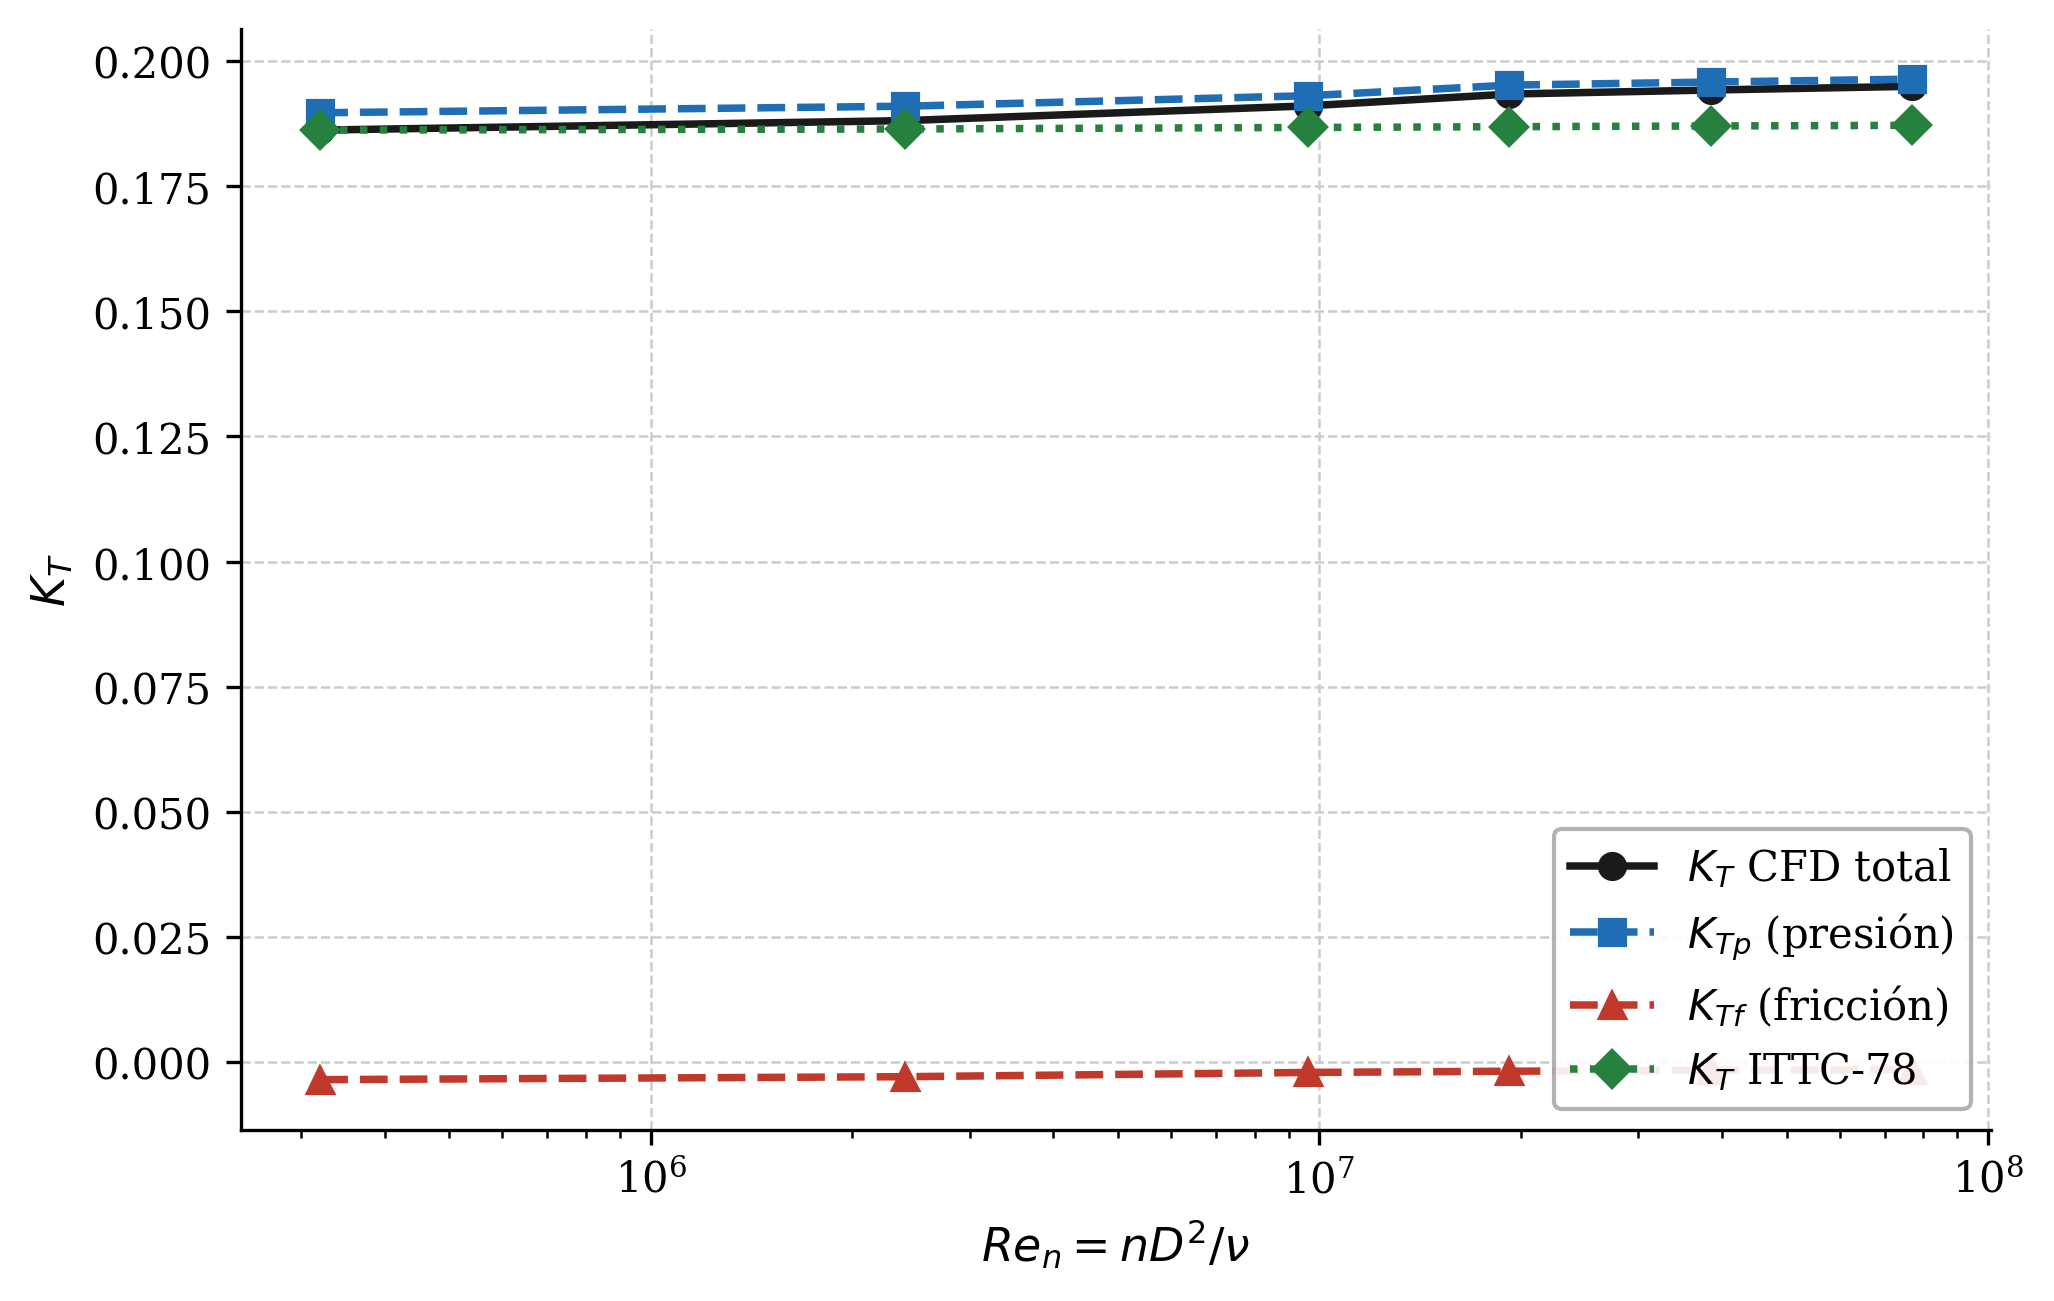
\includegraphics[width=0.75\textwidth]{images/fig1_Kt_Re.png}
\caption{Coeficientes $K_T$, $K_{Tp}$ y $K_{Tf}$ en función del número de Reynolds $Re_n = nD^2/\nu$ para el barrido de escala B4-60 a $J=0.5$. Se incluye la predicción del procedimiento ITTC-78 como referencia.}
\label{fig:kt_vs_re}
\end{figure}

\subsection{Descomposición friccional/presión ($\Delta K_{Tf}$, $\Delta K_{Tp}$, $\Delta K_{Qf}$, $\Delta K_{Qp}$)}
\label{sec:helices_descomposicion}

La descomposición de las fuerzas e integración de momentos que realiza OpenFOAM permite separar las contribuciones friccional y de presión a $K_T$ y $K_Q$ para cada escala. La Tabla~\ref{tab:delta_sweep_b460} presenta las variaciones acumuladas respecto a la referencia $D = 0.14$~m.

\begin{table}[htpb]
\centering
\caption{Variaciones de $K_T$ y $10K_Q$ respecto a $D=0.14$~m, descompuestas en contribuciones de presión y fricción. La columna $\Delta K_{Tp}/\Delta K_T$ indica la fracción del efecto de escala atribuible a la componente de presión.}
\label{tab:delta_sweep_b460}
\small
\begin{tabular}{cccccccc}
\hline
$D$ [m] & $\Delta K_T$ & $\Delta K_{Tp}$ & $\Delta K_{Tf}$ & $\frac{\Delta K_{Tp}}{\Delta K_T}$ & $10\Delta K_Q$ & $10\Delta K_{Qp}$ & $10\Delta K_{Qf}$ \\
\hline
$0.50$ & $+0.0019$ & $+0.0013$ & $+0.0006$ & $68.9\%$ & $-0.0054$ & $+0.0011$ & $-0.0065$ \\
$1.00$ & $+0.0048$ & $+0.0034$ & $+0.0014$ & $70.3\%$ & $-0.0104$ & $+0.0034$ & $-0.0137$ \\
$2.00$ & $+0.0072$ & $+0.0055$ & $+0.0017$ & $76.6\%$ & $-0.0095$ & $+0.0064$ & $-0.0159$ \\
$4.00$ & $+0.0080$ & $+0.0061$ & $+0.0019$ & $76.6\%$ & $-0.0103$ & $+0.0072$ & $-0.0176$ \\
$8.00$ & $+0.0087$ & $+0.0067$ & $+0.0020$ & $76.8\%$ & $-0.0109$ & $+0.0080$ & $-0.0190$ \\
\hline
\end{tabular}
\end{table}

El resultado más significativo de esta descomposición es que la componente de presión domina el efecto de escala en $K_T$: entre $D=1.0$ y $D=8.0$~m, la fracción $\Delta K_{Tp}/\Delta K_T$ se estabiliza en torno al $76$--$77\%$ (Figura~\ref{fig:delta_descomp}). Esto implica que aproximadamente tres cuartas partes del incremento de empuje al pasar de escala modelo a escala buque no provienen de la reducción de fricción, sino de cambios en la distribución de presiones sobre las palas asociados al adelgazamiento de la capa límite. En $K_Q$, el comportamiento es diferente: $\Delta K_{Qp}$ es positivo (el par de presión aumenta ligeramente con la escala) mientras que $\Delta K_{Qf}$ es negativo y de mayor magnitud, de modo que la reducción total de par está dominada por la componente friccional. Este comportamiento asimétrico entre empuje y par tiene implicaciones directas para la evaluación de los métodos de extrapolación, que se analizan en la sección siguiente.

\begin{figure}[htpb]
\centering
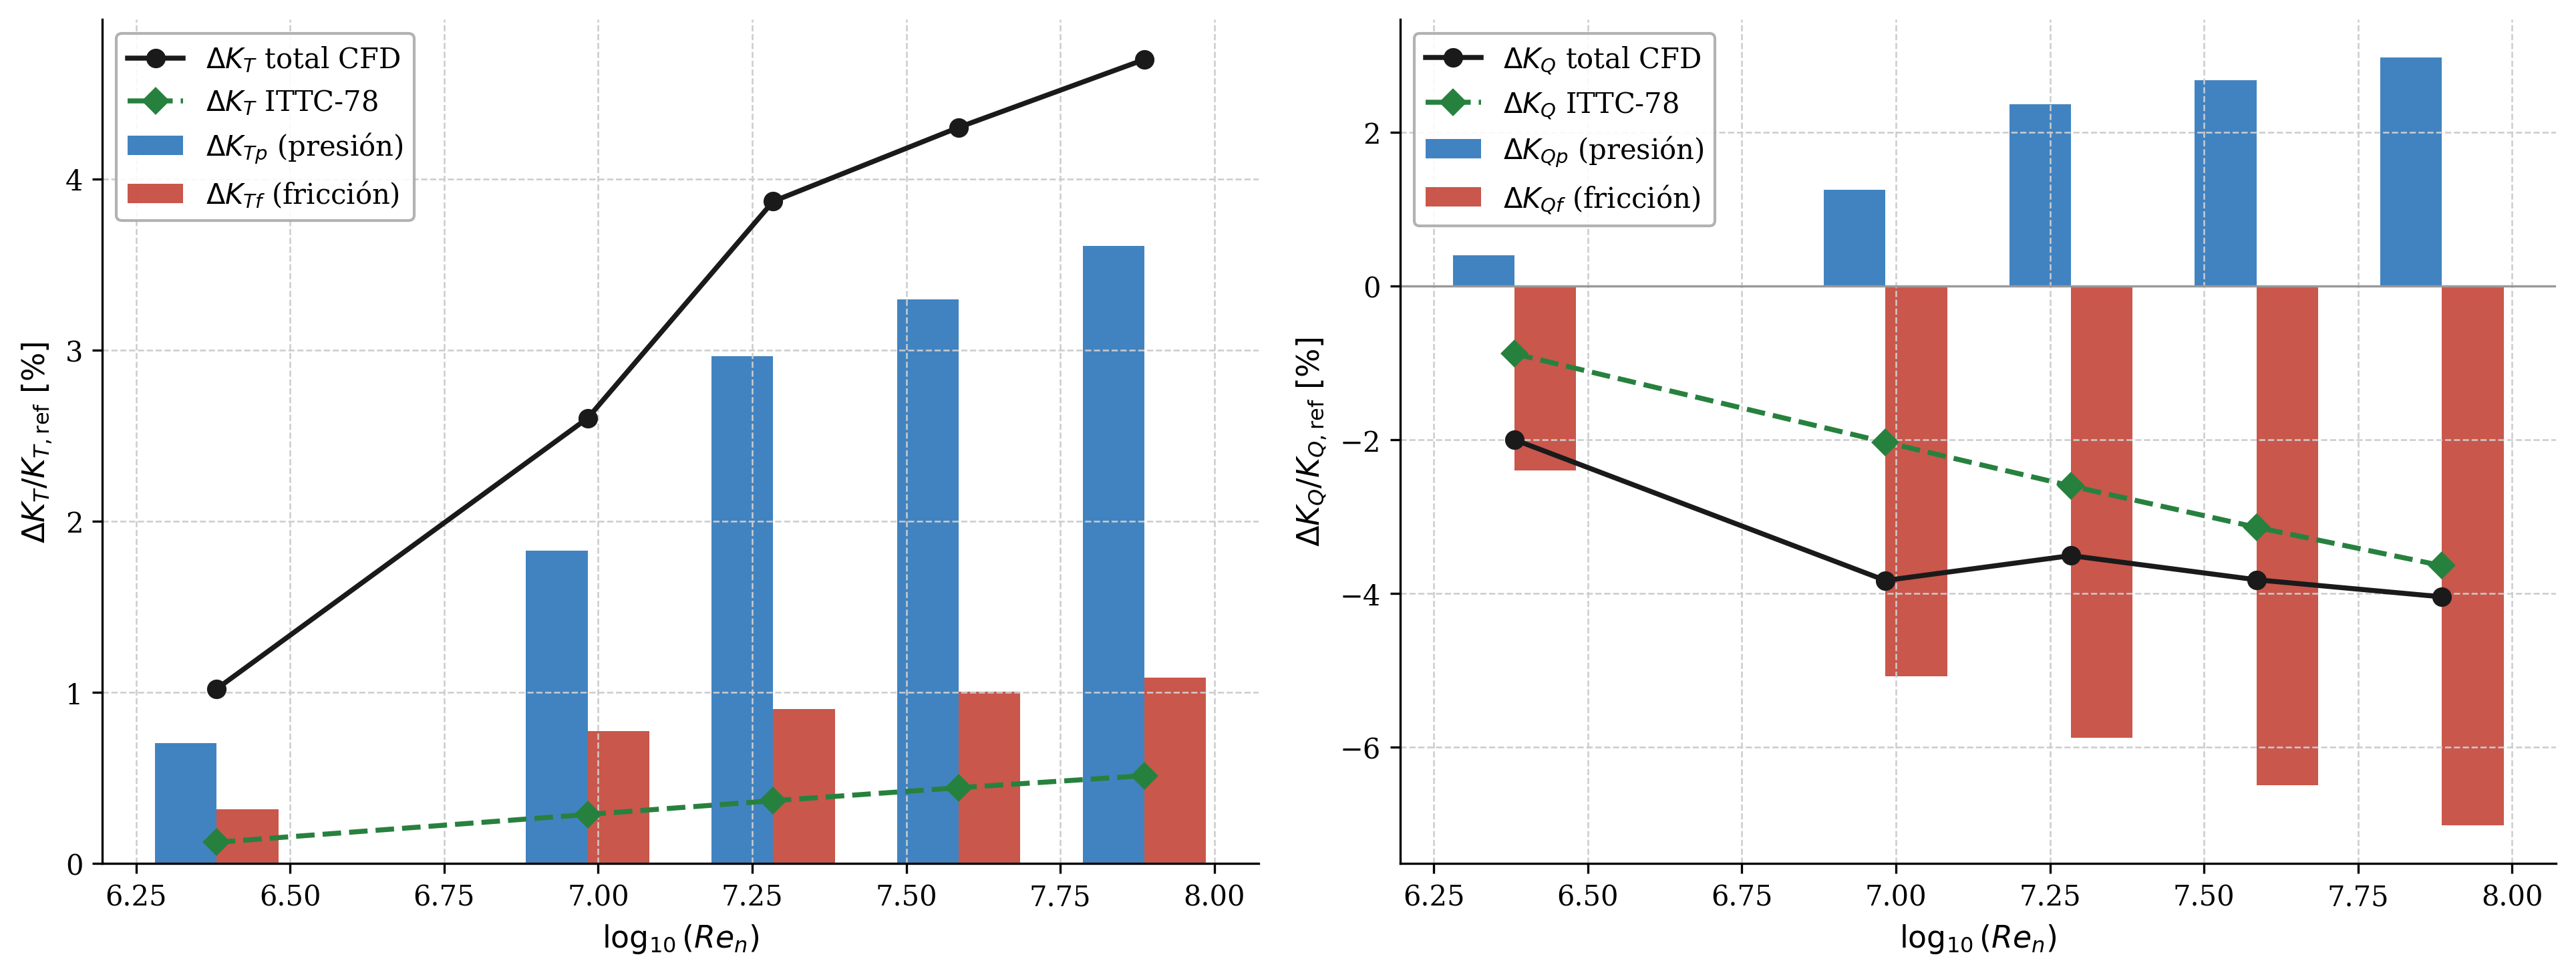
\includegraphics[width=0.95\textwidth]{images/fig2_delta_descomp.png}
\caption{Variación porcentual de $\Delta K_T$ (izquierda) y $\Delta K_Q$ (derecha) respecto al caso de referencia $D=0.14$~m, descompuesta en contribuciones de presión y fricción. Se incluye la predicción del ITTC-78.}
\label{fig:delta_descomp}
\end{figure}

% ============================================================
%  Subsección para insertar en la Sección 8.2 (Efectos de escala en la B4-60),
%  a continuación de \subsection{Descomposición friccional/presión ...}
%  (label sec:helices_descomposicion) y antes de
%  \subsection{Comparación con el procedimiento ITTC-78}.
%
%  NOTA (etiquetado de Reynolds):
%  Las figuras se rotulan con el Re_n = nD^2/nu REALIZADO de cada caso, calculado
%  con nu = 0.95653e-6 (la viscosidad real de las simulaciones). Los puntos del
%  barrido son Re_n ~ 1e4, 5e4, 1.44e5, 7.19e5, 1.44e6 y 2.5e6. Los nombres de
%  carpeta (1e5, 5e5, 1e6) NO coinciden con el Re_n realizado en tres casos, por
%  un nu inconsistente al fijar las rpm; por eso se etiqueta con el Re_n realizado.
%  Este barrido de campo (hasta Re_n ~ 2.5e6) es distinto del barrido de fuerzas
%  de la Tabla~\ref{tab:barrido_b460} (hasta Re_n ~ 7.7e7). Copiar los PNG a images/:
%    delta_cp_dorso.png, delta_cp_cara.png, radial_rms_dcp.png,
%    radial_rms_dcp_amp.png, cp_section_r07.png, cp_section_r09.png
% ============================================================
\subsection{Distribución superficial del efecto de escala en presión}
\label{sec:helices_campo_presion}
La descomposición de la Sección~\ref{sec:helices_descomposicion} establece, a partir de la integración de fuerzas, que alrededor de tres cuartas partes del incremento de empuje con la escala provienen de la componente de presión y no de la reducción de fricción. Ese resultado es, sin embargo, una magnitud integral: indica \emph{cuánto} pesa la presión, pero no \emph{dónde} sobre la pala se produce la redistribución ni cómo evoluciona con el número de Reynolds. Para esclarecer el mecanismo se analiza a continuación el campo de presión sobre la pala directamente, comparándolo entre escalas, a partir de un barrido de Reynolds dedicado de la B4-60 que abarca $Re_n$ desde $\sim\!10^{4}$ (escala modelo) hasta $\sim\!2.5\times10^{6}$. Este rango cubre el inicio y buena parte de la evolución del efecto de escala en régimen turbulento; como se muestra más abajo, la redistribución de presión se encuentra prácticamente saturada dentro de él, en consonancia con la estabilización de la fracción $\Delta K_{Tp}/\Delta K_T$ observada en la Tabla~\ref{tab:delta_sweep_b460}.
El coeficiente de presión sobre la pala se define, siguiendo la convención habitual para propulsores, respecto de la presión dinámica construida con la velocidad resultante en la sección de referencia a $r/R=0.7$,
\begin{equation}
C_p = \frac{p - p_\infty}{\tfrac{1}{2}\rho\,V_{0.7R}^2},
\qquad
V_{0.7R}^2 = V_a^2 + \left(0.7\,\pi n D\right)^2,
\qquad
V_a = J\,n\,D,
\label{eq:cp_helice}
\end{equation}
de modo que $C_p$ resulta adimensional y comparable entre escalas. El efecto de escala local se caracteriza mediante el campo de diferencia
\begin{equation}
\Delta C_p = C_{p}(Re_n) - C_{p}(Re_{n,\mathrm{ref}}),
\label{eq:dcp_helice}
\end{equation}
evaluado sobre la geometría de la escala de referencia (escala modelo). Como todas las mallas se obtienen escalando uniformemente una única malla base, al adimensionalizar las coordenadas por el diámetro las superficies de dos escalas cualesquiera se superponen de forma exacta, y la diferencia de la Ecuación~\ref{eq:dcp_helice} se calcula punto a punto sin interpolación ni ambigüedad. Cabe destacar que las tres métricas de campo empleadas en esta subsección --el mapa de $\Delta C_p$, su perfil radial y su amplitud-- son puramente descriptivas: cuantifican la magnitud y la localización de la redistribución de presión, y no reconstruyen fuerzas. La contribución neta de la presión al empuje y al par sigue siendo la reportada por la integración de OpenFOAM en la Sección~\ref{sec:helices_descomposicion}.
\paragraph{Distribución sobre la pala.} La Figura~\ref{fig:dcp_map} muestra el campo $\Delta C_p$ entre la escala modelo y la mayor escala del barrido ($Re_n\approx 2.5\times10^{6}$), sobre el dorso (lado de succión) y la cara (lado de presión). El contraste entre ambos lados es marcado. La cara permanece casi invariable con la escala, salvo una franja delgada en las proximidades del borde de ataque hacia la punta. El dorso, en cambio, concentra prácticamente toda la redistribución: la succión se profundiza ($\Delta C_p<0$) a lo largo del borde de ataque --de forma más intensa hacia la punta-- mientras que hacia el borde de salida y la zona media-externa la presión se recupera ($\Delta C_p>0$). Este patrón es la firma esperada del adelgazamiento de la capa límite al aumentar $Re_n$: un pico de succión de borde de ataque más marcado y una mejor recuperación de presión aguas abajo. El resultado localiza espacialmente la componente de presión que la descomposición de fuerzas cuantifica de forma global y confirma que actúa esencialmente sobre el lado de succión. Los valores extremos de $\Delta C_p$ se ubican en la esquina punta--borde de ataque; conviene recordar que esa zona, junto con el borde de salida, es la de mayor sensibilidad a la discretización geométrica del extremo de pala, por lo que su magnitud puntual no debe sobreinterpretarse, si bien la redistribución en el cuerpo de la pala es robusta.
\begin{figure}[htpb]
\centering
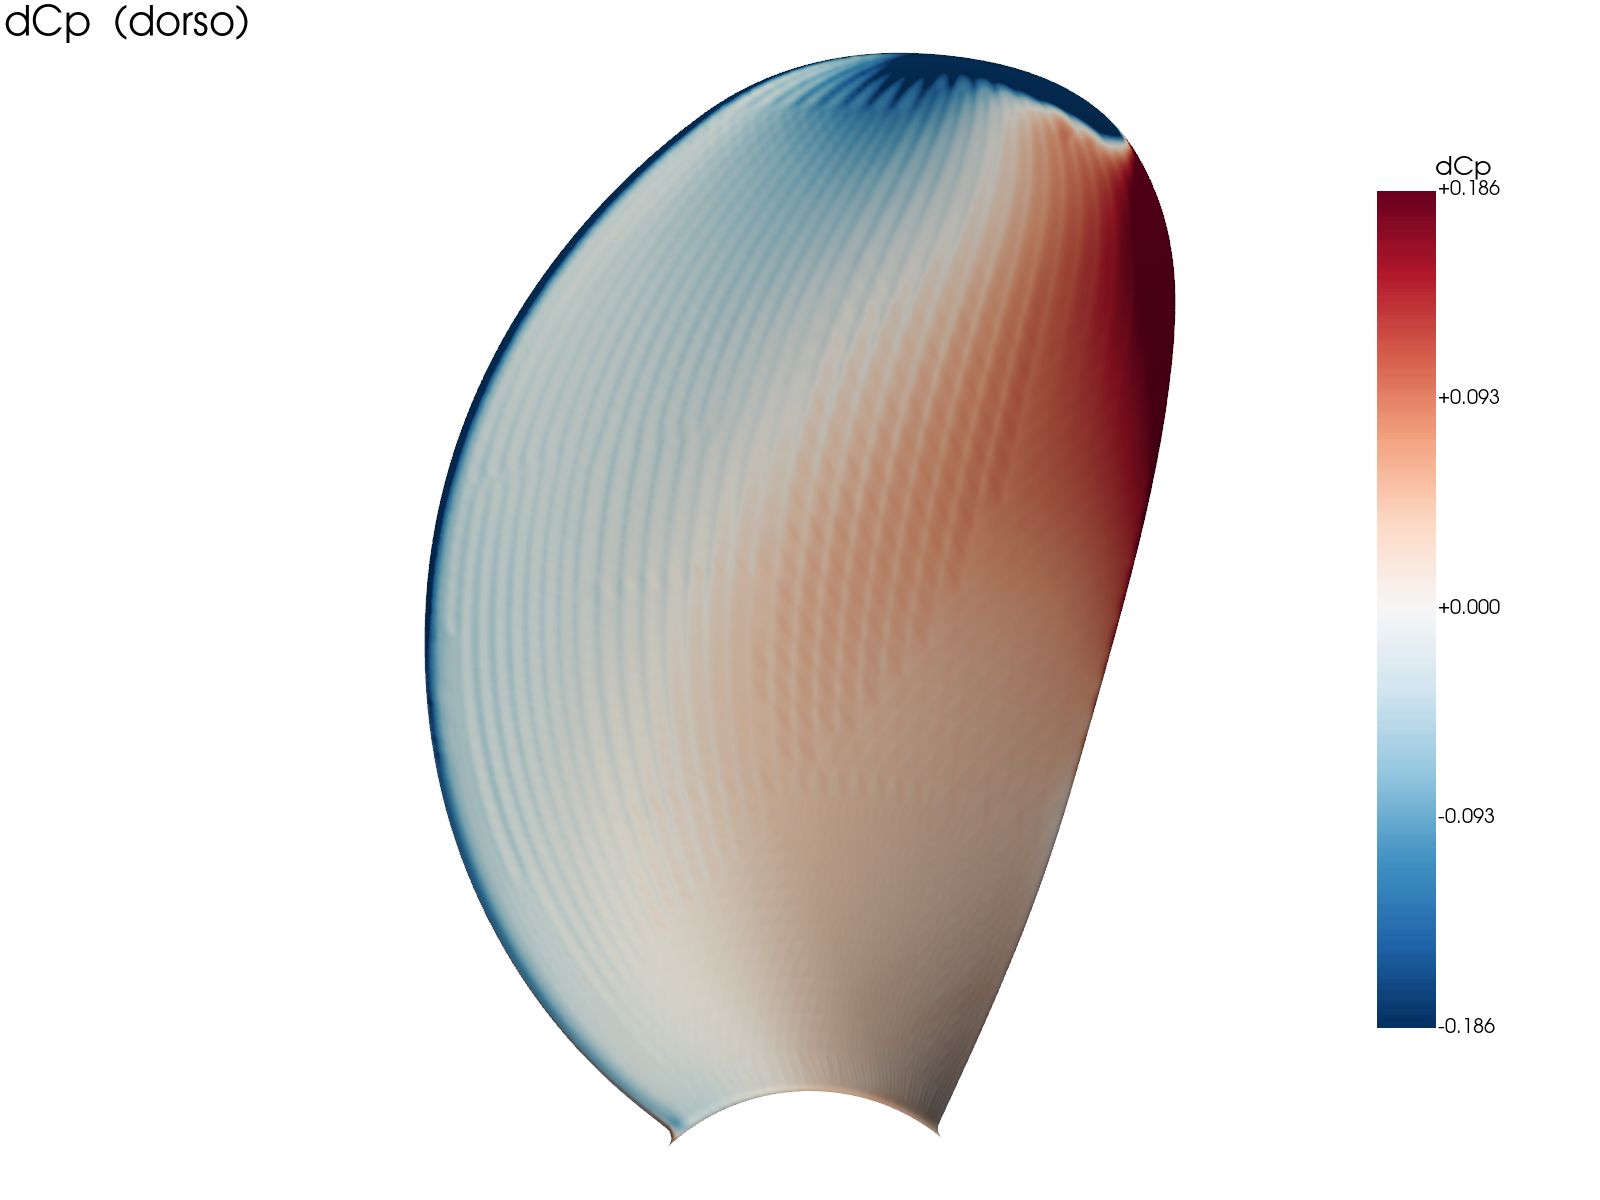
\includegraphics[width=0.48\textwidth]{images/delta_cp_dorso.png}\hfill
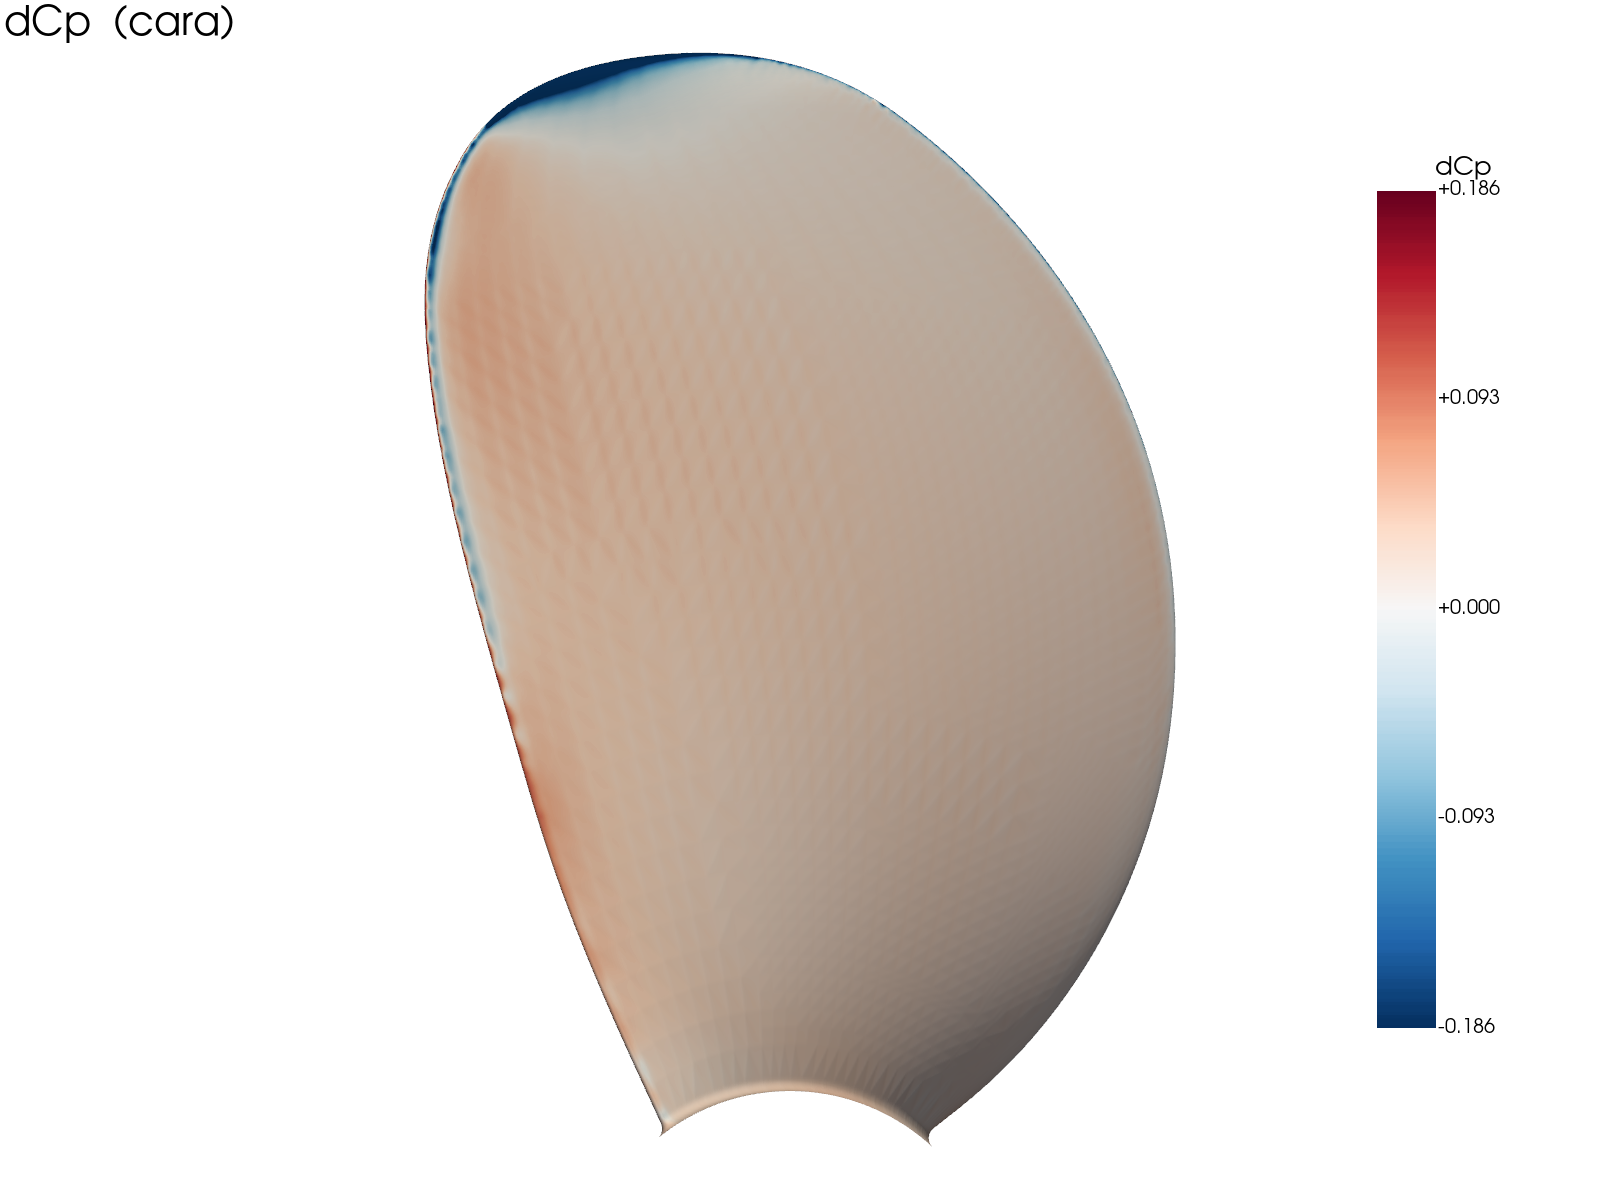
\includegraphics[width=0.48\textwidth]{images/delta_cp_cara.png}
\caption{Campo de diferencia $\Delta C_p = C_p(Re_n) - C_p(Re_{n,\mathrm{ref}})$ entre la escala modelo y $Re_n\approx 2.5\times10^{6}$, sobre el dorso (izquierda, lado de succión) y la cara (derecha, lado de presión) de la pala B4-60. El rango de color es simétrico y se recorta al percentil 98 de $|\Delta C_p|$ para evitar que los extremos de punta y bordes dominen la escala.}
\label{fig:dcp_map}
\end{figure}
\paragraph{Distribución radial.} Para cuantificar la observación anterior, el mapa se colapsa a una curva radial mediante el valor cuadrático medio de $\Delta C_p$ pesado por el área de celda en bandas de radio constante,
\begin{equation}
\mathrm{RMS}_{\Delta C_p}(r/R) = \sqrt{\frac{\sum_i \Delta C_{p,i}^{\,2}\,|A_i|}{\sum_i |A_i|}},
\label{eq:rms_dcp}
\end{equation}
donde la suma recorre las celdas de cada banda. La Figura~\ref{fig:dcp_radial} presenta esta curva para todas las escalas del barrido. En todo el tramo interior y medio de la pala la amplitud del efecto crece de forma suave y monótona hacia la punta, con las escalas perfectamente ordenadas por $Re_n$: la redistribución de presión es despreciable en la raíz y se intensifica hacia la mitad externa, coherentemente con lo observado en el mapa. Se excluye del gráfico la región $r/R>0.95$, donde el vórtice de punta y la discretización del borde dominan la señal y no son representativos de la redistribución asociada a la capa límite.
\begin{figure}[htpb]
\centering
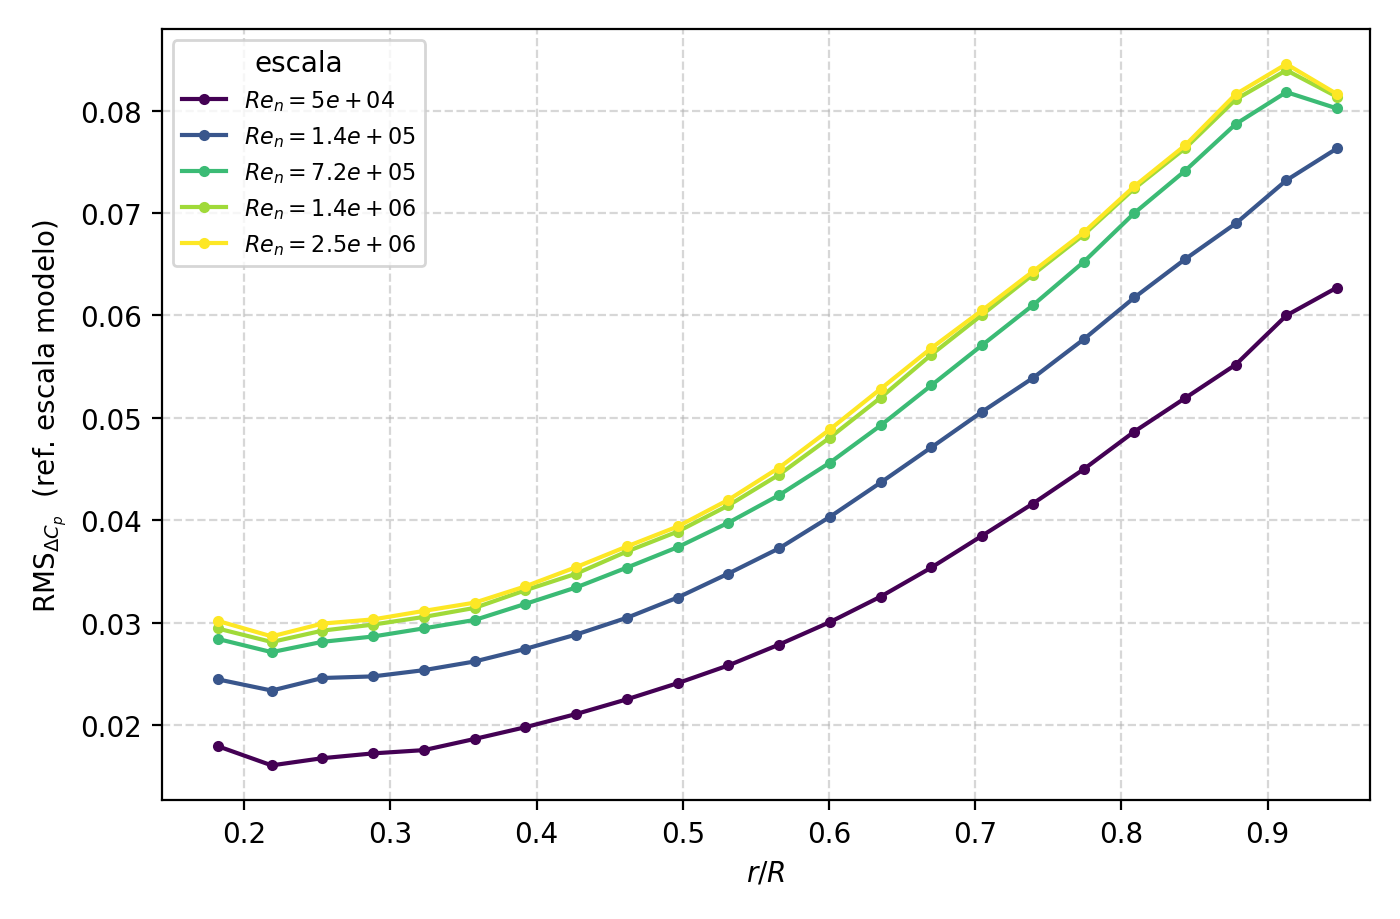
\includegraphics[width=0.75\textwidth]{images/radial_rms_dcp.png}
\caption{Valor cuadrático medio radial de $\Delta C_p$ (Ecuación~\ref{eq:rms_dcp}), referido a la escala modelo, en función de $r/R$ para las escalas del barrido. Se excluye $r/R>0.95$ (vórtice de punta y borde, sensibles a la discretización).}
\label{fig:dcp_radial}
\end{figure}
\paragraph{Convergencia con el número de Reynolds.} La Figura~\ref{fig:dcp_amp} colapsa cada campo a una única amplitud --el RMS de $\Delta C_p$ pesado por área sobre la pala hasta $r/R<0.95$-- y la representa en función de $Re_n$. La curva, anclada en cero en la escala modelo por definición, crece empinadamente en el primer tramo y se aplana hacia los Reynolds altos: más de la mitad de la redistribución de presión ya está presente en $Re_n\sim 5\times10^{4}$ y del orden del $95\%$ hacia $Re_n\sim 7\times10^{5}$, con los dos puntos de mayor Reynolds prácticamente indistinguibles. Este comportamiento de saturación es consistente con la estabilización de la fracción $\Delta K_{Tp}/\Delta K_T$ en torno al $76$--$77\%$ observada en la descomposición de fuerzas (Tabla~\ref{tab:delta_sweep_b460}) a partir de $D\gtrsim 1$~m, e implica que la mayor parte del efecto de escala en presión se alcanza a Reynolds moderados. Debe subrayarse que esta amplitud es una medida sin signo de la \emph{magnitud} de la redistribución del campo, no de su aporte neto al empuje; este último es el $\Delta K_{Tp}$ de la Sección~\ref{sec:helices_descomposicion}.
\begin{figure}[htpb]
\centering
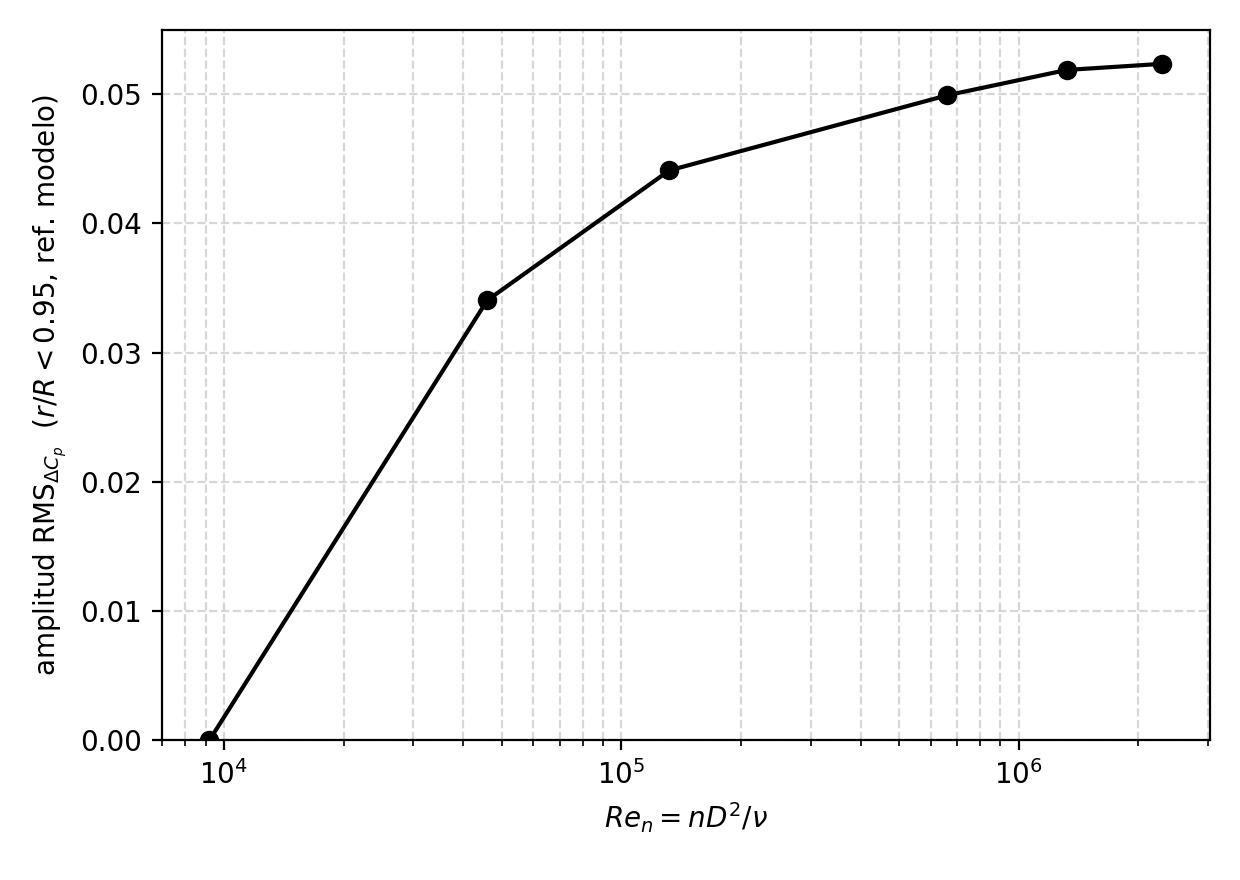
\includegraphics[width=0.7\textwidth]{images/radial_rms_dcp_amp.png}
\caption{Amplitud global de la redistribución de presión (RMS de $\Delta C_p$ pesado por área, $r/R<0.95$, referido a la escala modelo) en función de $Re_n = nD^2/\nu$. La curva evidencia la saturación del efecto de escala en presión hacia $Re_n\sim10^{6}$.}
\label{fig:dcp_amp}
\end{figure}
\paragraph{Mecanismo seccional.} Finalmente, la Figura~\ref{fig:cp_secciones} presenta la distribución de $C_p$ en función de la coordenada de cuerda $x/c$ en dos secciones representativas, $r/R=0.7$ y $r/R=0.9$, para todas las escalas. Cada sección se obtiene como la isolínea de radio constante sobre la pala, un corte puramente geométrico. En el dorso, el pico de succión de borde de ataque se profundiza sistemáticamente al aumentar $Re_n$ --desde la escala modelo, de pico más chato, hasta las escalas mayores-- y hacia el borde de salida las curvas de mayor Reynolds caen por debajo de la de escala modelo, reflejando la mejor recuperación de presión de la capa límite adelgazada. El efecto es más pronunciado en $r/R=0.9$ que en $r/R=0.7$, en concordancia con la concentración hacia la punta ya evidenciada en las Figuras~\ref{fig:dcp_map} y \ref{fig:dcp_radial}. En la cara, por el contrario, las curvas de las distintas escalas se superponen casi por completo, confirmando que la redistribución de presión reside casi enteramente en el lado de succión. Este diagnóstico seccional es el análogo, como estudio de convergencia con la escala, del que se aplica a la hélice de la Sección~\ref{sec:helice_coreana} para el mecanismo transicional.
\begin{figure}[htpb]
\centering
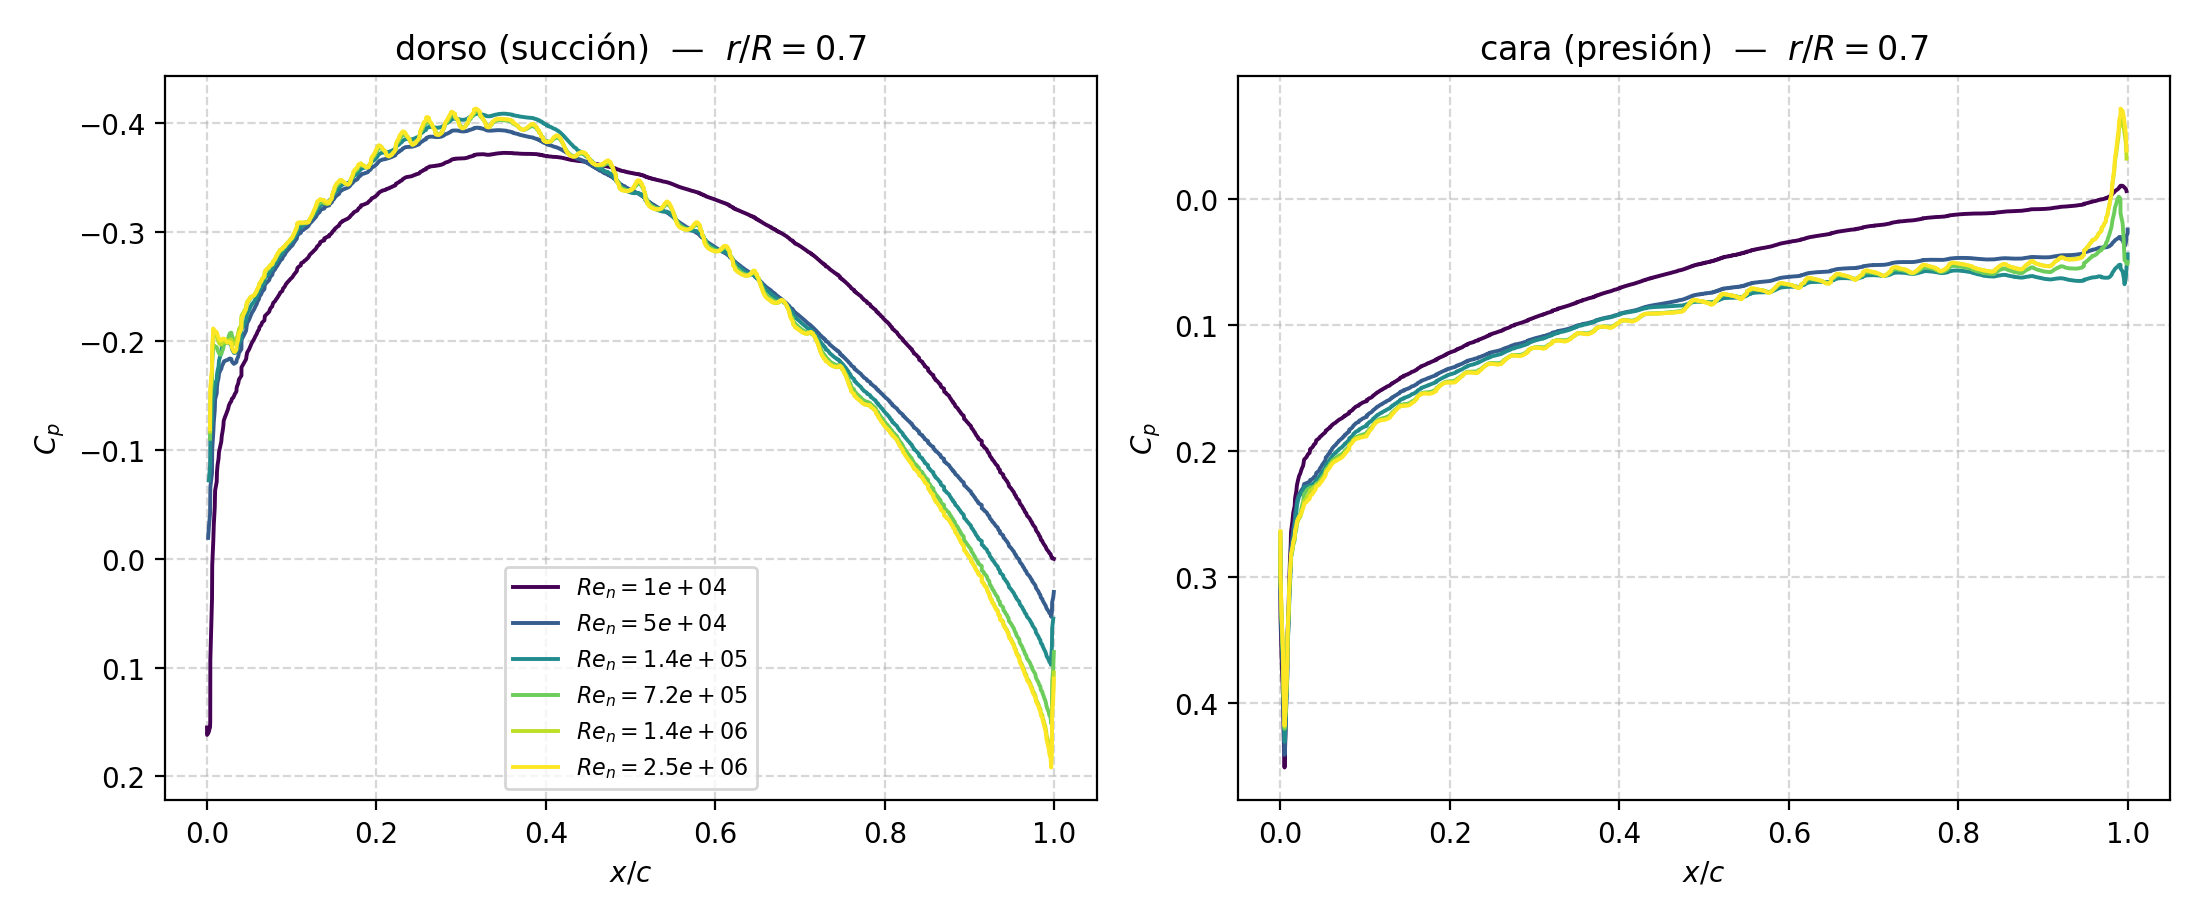
\includegraphics[width=0.92\textwidth]{images/cp_section_r07.png}\\[2pt]
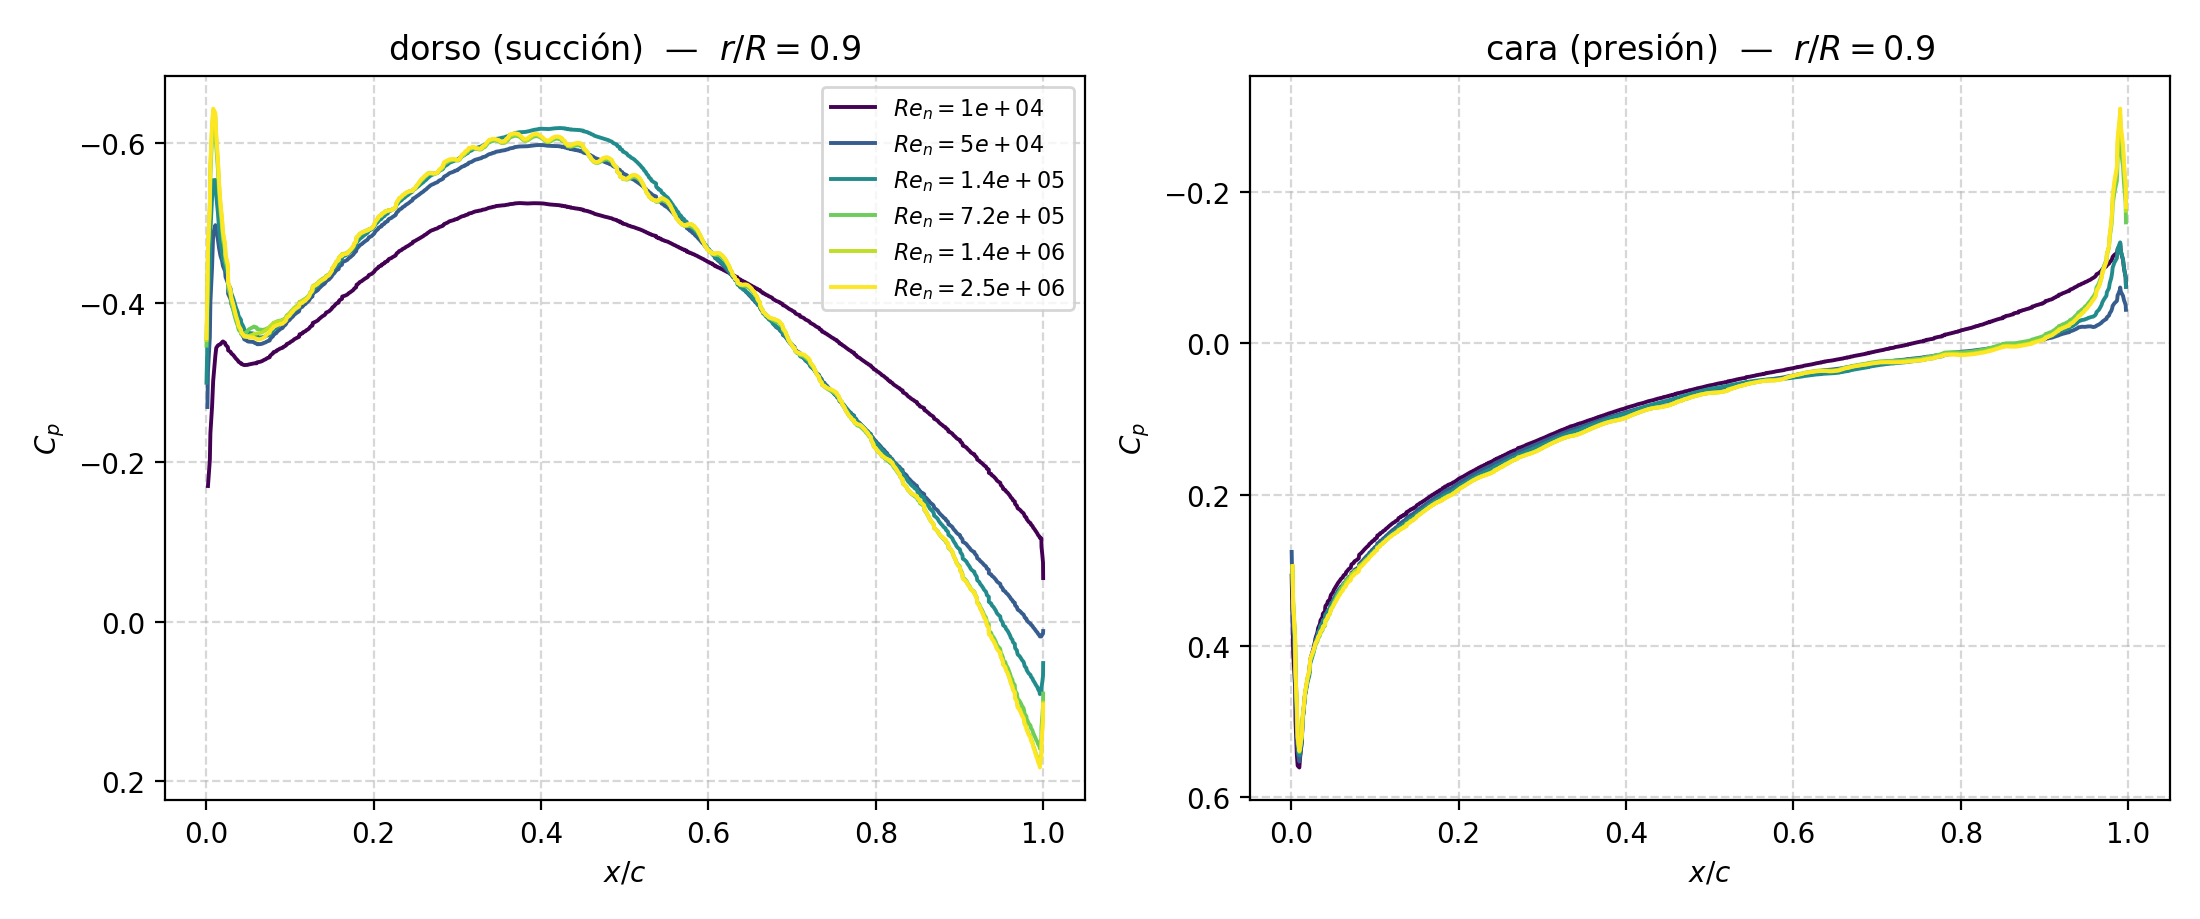
\includegraphics[width=0.92\textwidth]{images/cp_section_r09.png}
\caption{Distribución de $C_p$ a lo largo de la cuerda ($x/c$) en las secciones $r/R=0.7$ (arriba) y $r/R=0.9$ (abajo), para las escalas del barrido, separada en dorso (succión, izquierda) y cara (presión, derecha). El eje de $C_p$ está invertido (succión hacia arriba). Se aprecia el pico de succión de borde de ataque profundizándose con $Re_n$ sobre el dorso y la escasa sensibilidad de la cara.}
\label{fig:cp_secciones}
\end{figure}
En conjunto, las Figuras~\ref{fig:dcp_map}--\ref{fig:cp_secciones} corroboran, a nivel del campo de presión, el resultado obtenido por integración de fuerzas: el efecto de escala en régimen turbulento sobre la B4-60 posee una componente de presión dominante y espacialmente coherente, que el procedimiento ITTC-78 --al suponer $\Delta K_{Tp}=0$-- ignora por completo. Más aún, permiten precisar su naturaleza: se trata de una redistribución concentrada en el lado de succión de la mitad externa de la pala, que se intensifica hacia la punta y que satura a Reynolds moderados. Esta caracterización espacial refuerza la conclusión, desarrollada en la sección siguiente, de que la corrección puramente friccional del ITTC-78 es estructuralmente incapaz de capturar el efecto de escala de esta hélice.

\subsection{Comparación con el procedimiento ITTC-78}
\label{sec:helices_ittc78}

El procedimiento ITTC-78 corrige los coeficientes hidrodinámicos de modelo a escala buque mediante la diferencia de coeficiente de fricción de placa plana $\Delta C_D$ evaluada a $r/R = 0.75$, según las expresiones presentadas en la Sección~\ref{sec:ittc78_helices_metodo}. Esta corrección asume implícitamente que el efecto de escala es de naturaleza puramente friccional, es decir, que $\Delta K_{Tp} = 0$. Los resultados del CFD demuestran que esta hipótesis es incorrecta para la B4-60.

La Tabla~\ref{tab:ittc_vs_cfd} compara las predicciones del ITTC-78 y del CFD para $D = 8.0$~m, tomando $D = 0.14$~m como referencia de modelo.

\begin{table}[htpb]
\centering
\caption{Comparación entre ITTC-78 y CFD a $D = 8.0$~m ($J = 0.5$), tomando $D = 0.14$~m como referencia.}
\label{tab:ittc_vs_cfd}
\begin{tabular}{lccc}
\hline
 & ITTC-78 & CFD SST & Diferencia \\
\hline
$K_T$   & $0.1862$ & $0.1949$ & $+0.0087$ $(+4.7\%)$ \\
$10K_Q$ & $0.2618$ & $0.2593$ & $-0.0025$ $(-1.0\%)$ \\
$\eta_0$ & $0.5540$ & $0.5982$ & $+0.0442$ $(+8.0\%)$ \\
\hline
\end{tabular}
\end{table}

El ITTC-78 subestima $K_T$ en $+4.7\%$ respecto al CFD a escala buque, precisamente porque no contempla el incremento de la componente de presión. Para $10K_Q$ la diferencia es menor ($-1.0\%$), dado que las contribuciones friccional y de presión evolucionan en sentidos opuestos y se compensan parcialmente. El efecto acumulado sobre la eficiencia es significativo: el ITTC-78 predice $\eta_0 = 0.554$ frente a $\eta_0 = 0.598$ del CFD, una diferencia de $+8.0\%$ que representaría una subestimación relevante en el diseño de la instalación propulsora. Las Figuras~\ref{fig:gap_fraccion} y~\ref{fig:delta_vs_D} sintetizan gráficamente esta comparación: la primera muestra la brecha $K_{T,\mathrm{CFD}}-K_{T,\mathrm{ITTC}}$ en función del diámetro y la fracción del efecto de escala atribuible a la presión frente a otras geometrías, y la segunda, la variación de $\Delta K_T$ y $10\,\Delta K_Q$ con el diámetro descompuesta en presión y fricción, junto con la predicción del ITTC-78.

\begin{figure}[htpb]
\centering
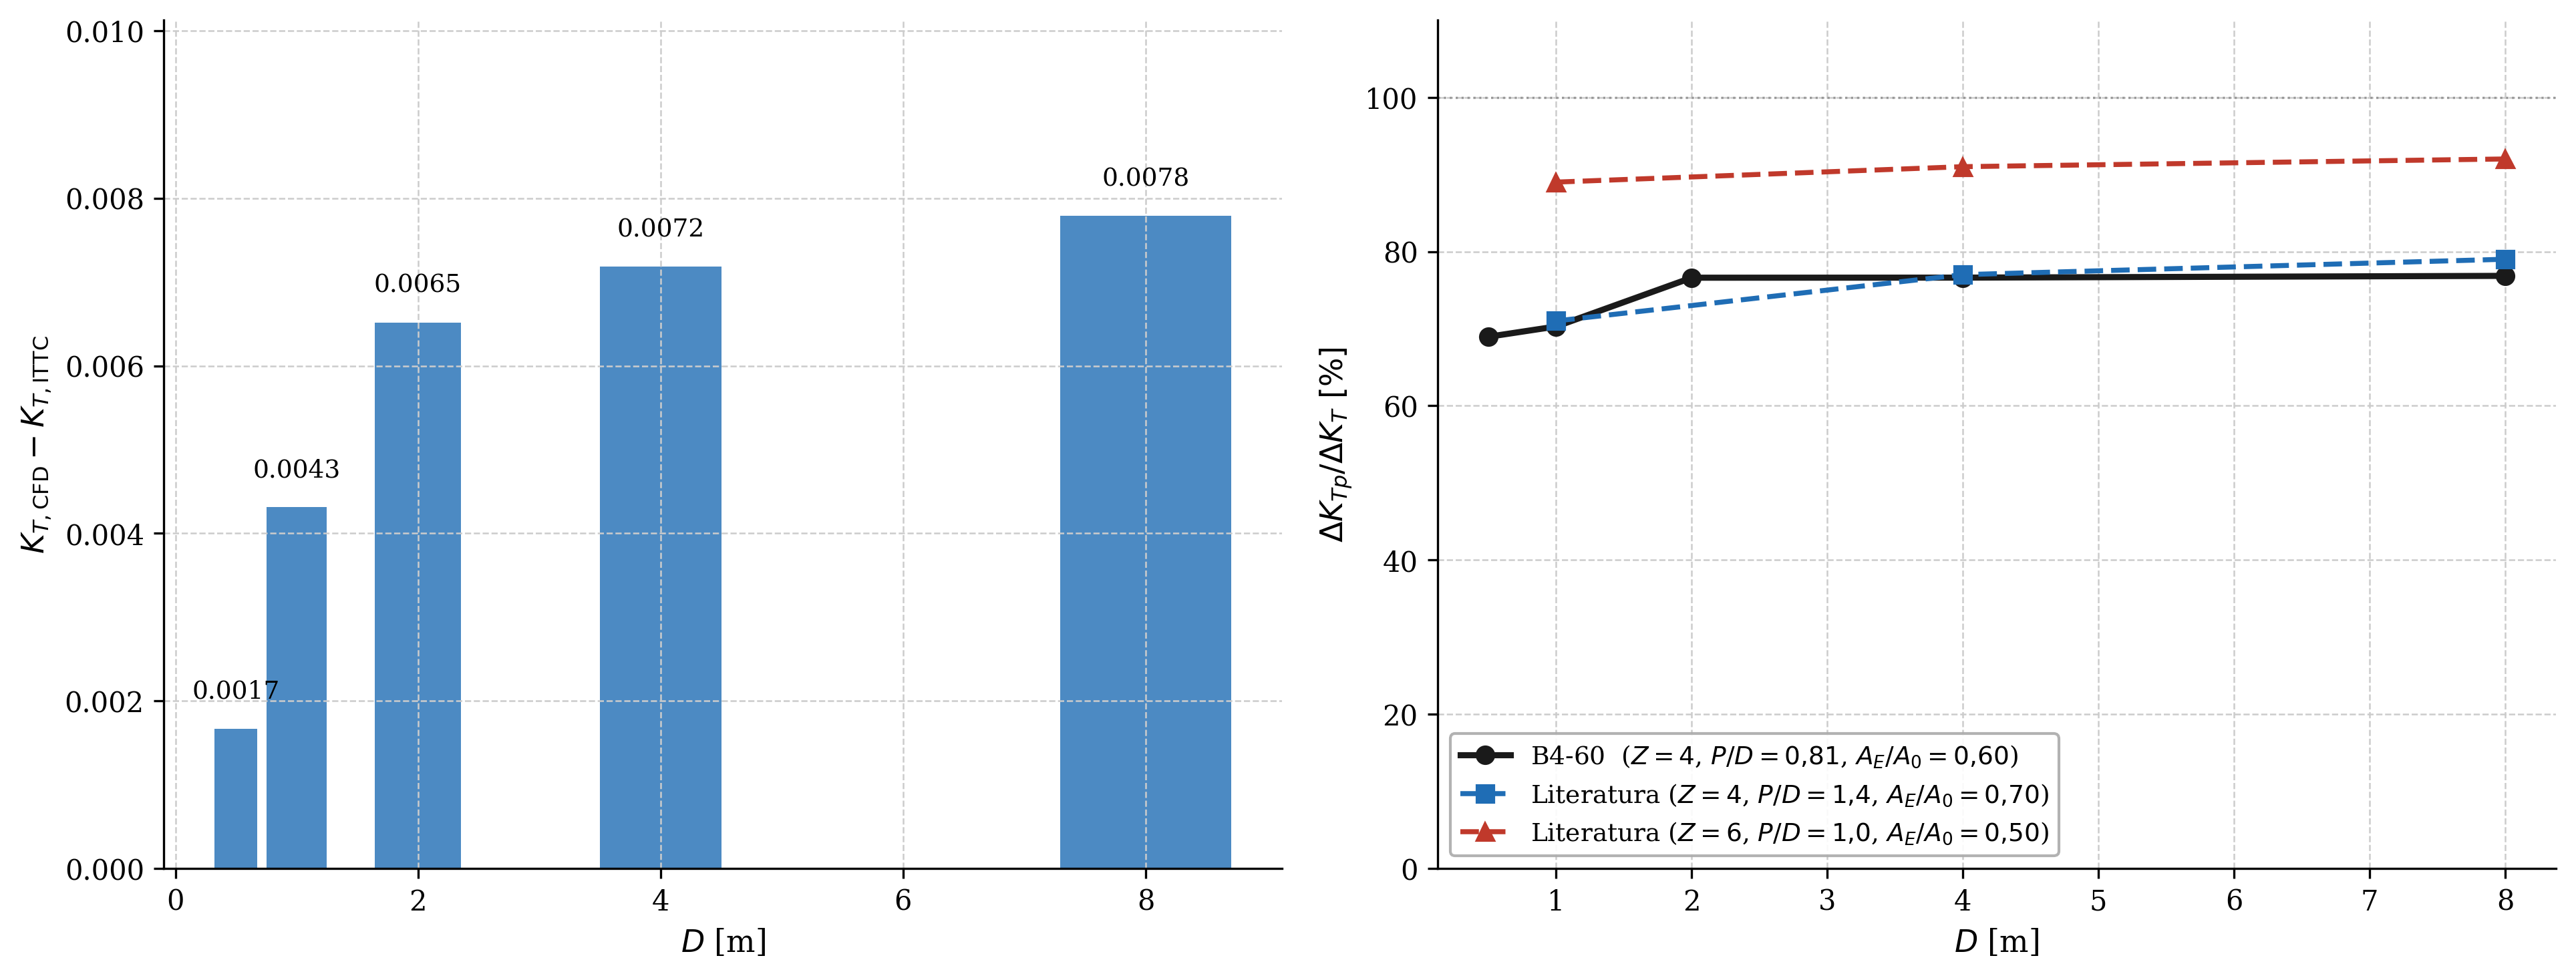
\includegraphics[width=0.95\textwidth]{images/fig4_gap_fraccion.png}
\caption{Izquierda: diferencia $K_{T,\mathrm{CFD}} - K_{T,\mathrm{ITTC}}$ en función del diámetro. Derecha: fracción del efecto de escala en $K_T$ atribuible a la componente de presión ($\Delta K_{Tp}/\Delta K_T$), comparada con datos de la literatura para otras geometrías.}
\label{fig:gap_fraccion}
\end{figure}

\begin{figure}[htpb]
\centering
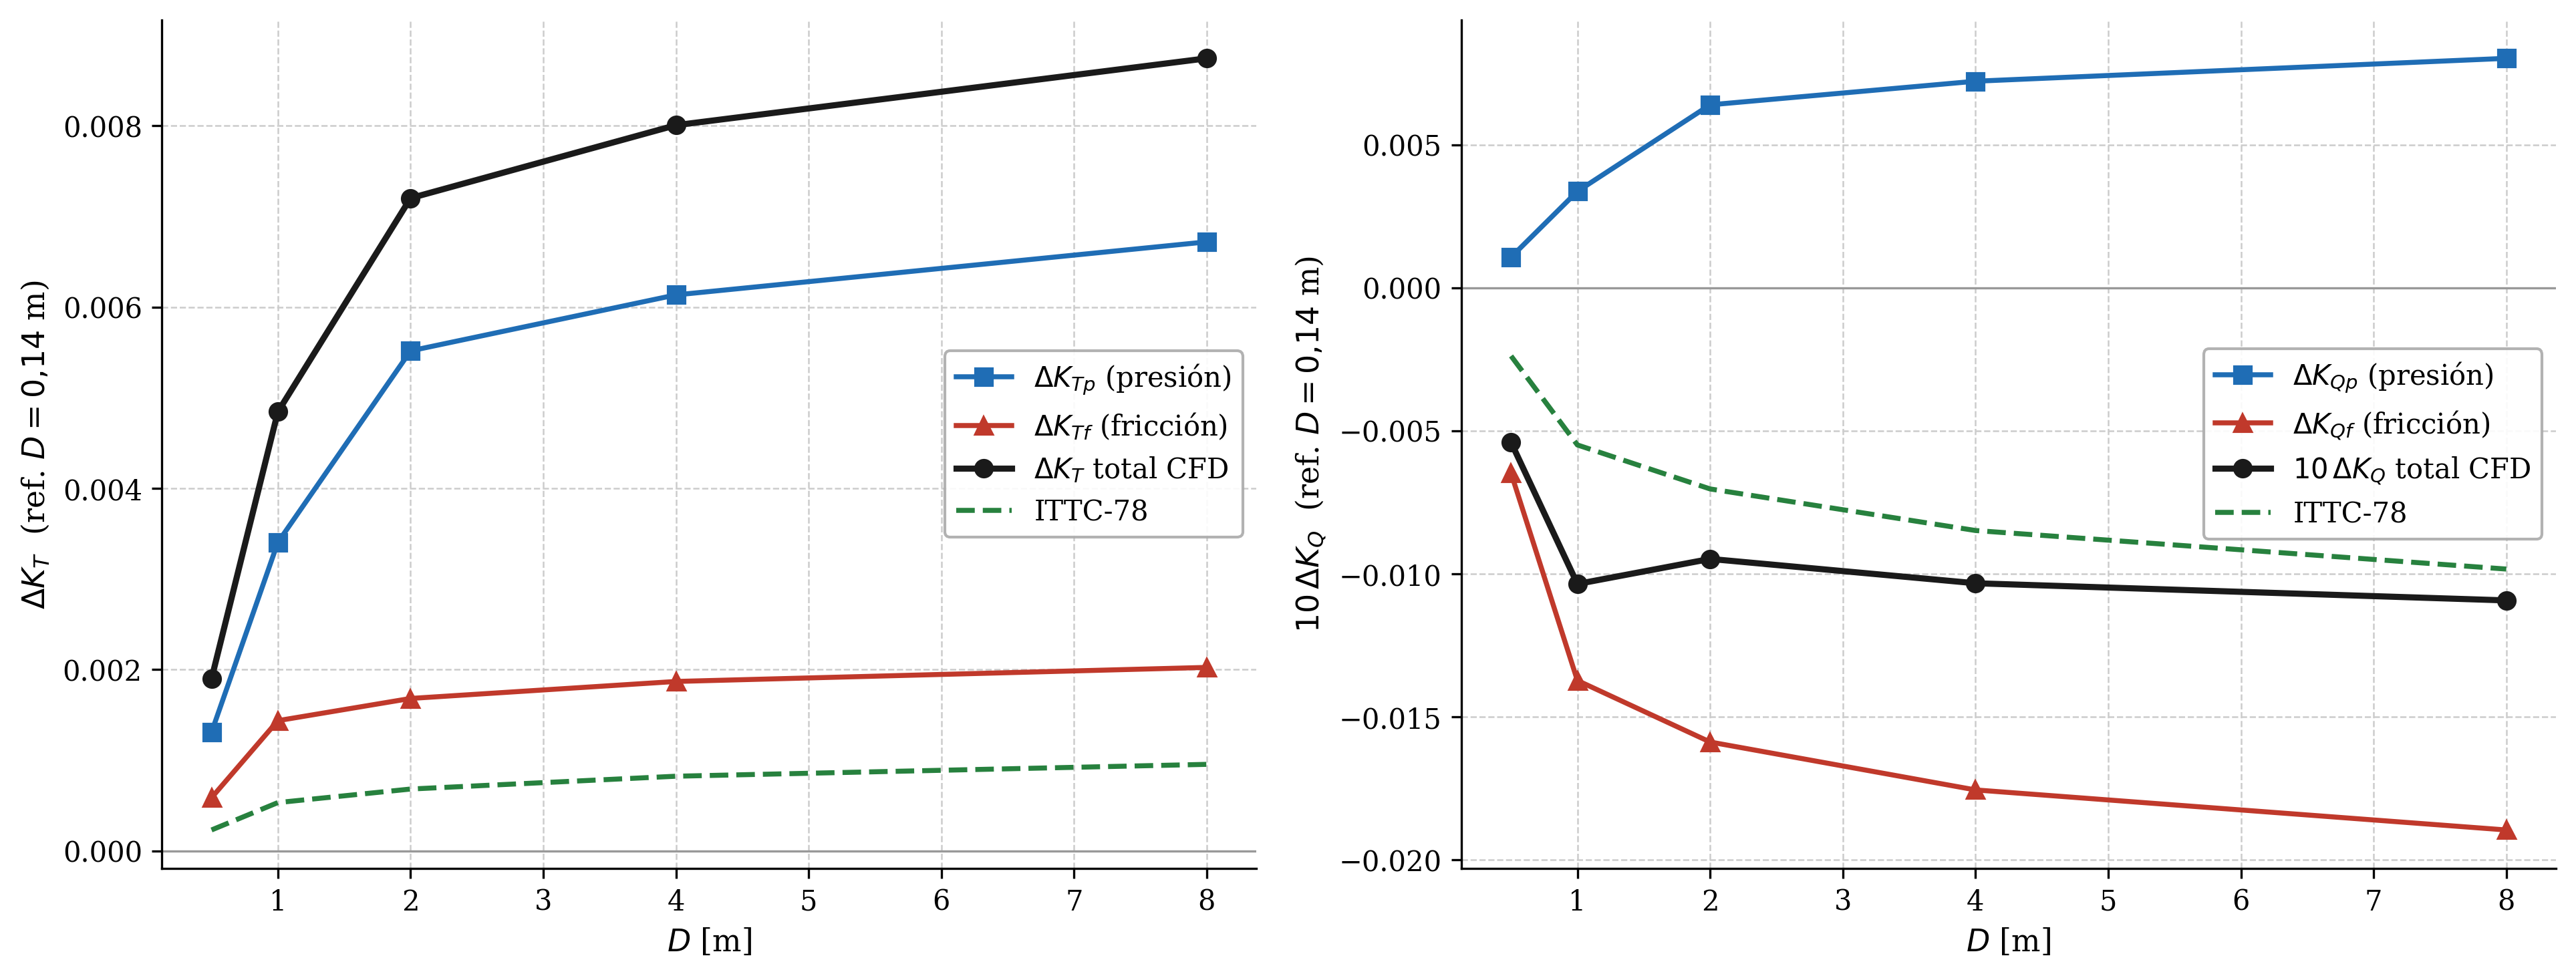
\includegraphics[width=0.95\textwidth]{images/fig3_delta_vs_D.png}
\caption{Variación de $\Delta K_T$ (izquierda) y $10\,\Delta K_Q$ (derecha) en función del diámetro, con descomposición en componentes de presión y fricción. Se incluye la predicción del ITTC-78.}
\label{fig:delta_vs_D}
\end{figure}

\subsection{Eficiencia en escala buque: comparación de métodos}
\label{sec:helices_eficiencia}

La Figura~\ref{fig:eficiencia_metodos} compara la evolución de $\eta_0$ con $Re_n$ para tres alternativas de extrapolación: el procedimiento ITTC-78 (M1), el CFD SST directo (M2) y la aplicación sin corrección del diagrama de modelo (M3). En $Re_n \approx 3.2 \times 10^5$ (D=0.14~m, escala modelo) los tres métodos coinciden por definición. A medida que $Re_n$ crece, M2 y M1 divergen progresivamente: a $D=8.0$~m ($Re_n \approx 7.7 \times 10^7$) el CFD predice un incremento de eficiencia de $+9.1\%$ respecto al modelo, mientras que el ITTC-78 solo estima $+1.1\%$. La diferencia entre ambos métodos, de $8.0$ puntos porcentuales a la mayor escala analizada, refleja la contribución ignorada de la componente de presión al efecto de escala.

\begin{figure}[htpb]
\centering
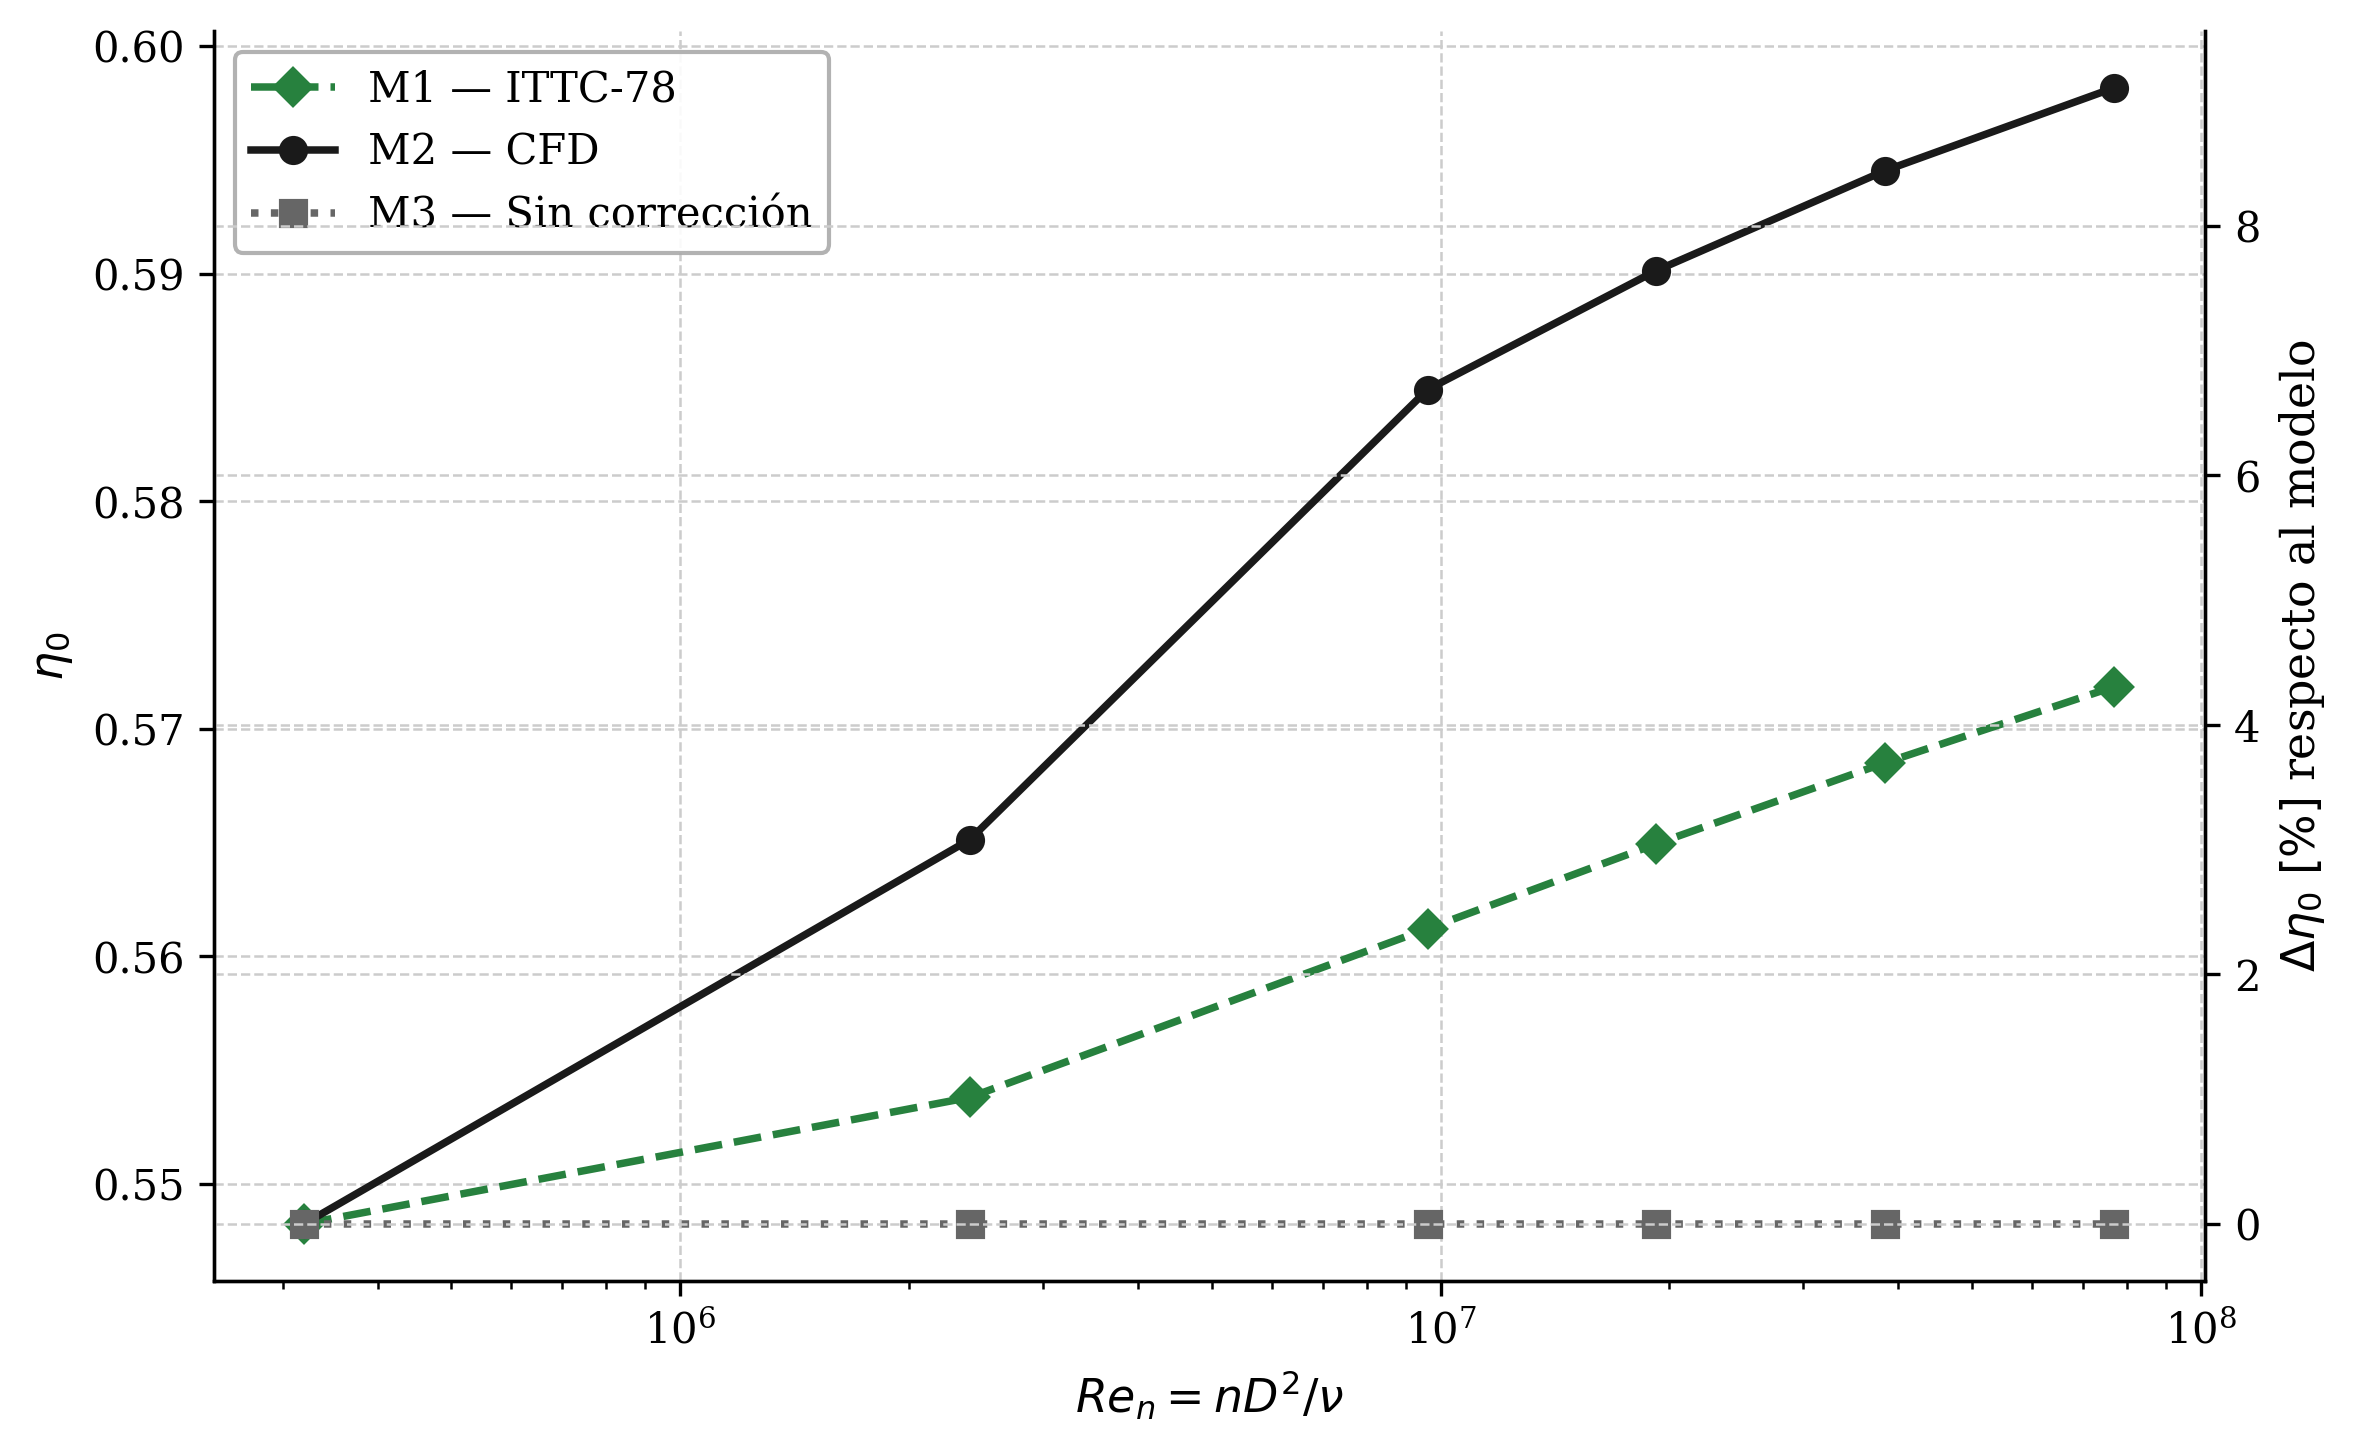
\includegraphics[width=0.95\textwidth]{images/fig2b_eficiencia.png}
\caption{Eficiencia en aguas abiertas $\eta_0$ (izquierda) y variación porcentual $\Delta\eta_0$ respecto al modelo (derecha) en función de $Re_n$, para los métodos ITTC-78 (M1), CFD SST (M2) y sin corrección (M3). Hélice B4-60, $J = 0.5$.}
\label{fig:eficiencia_metodos}
\end{figure}



\subsection{Conclusiones parciales}

El barrido de escala de la hélice B4-60, realizado en régimen completamente
turbulento entre $D=0.14$ y $8.0$~m, muestra que el efecto de escala sobre sus
coeficientes hidrodinámicos no es de naturaleza puramente friccional. El empuje crece
de forma monótona con el número de Reynolds ($\Delta K_T=+4.7\%$) y el par disminuye
($-4.1\%$), lo que se traduce en una ganancia de eficiencia en aguas abiertas de
$+9.1\%$ a la mayor escala (Secciones~\ref{sec:helices_sweep}
y~\ref{sec:helices_kt_kq_re}). La descomposición directa de fuerzas revela que ese
aumento de empuje está dominado por la presión: la fracción $\Delta K_{Tp}/\Delta K_T$
se estabiliza en torno al $76$--$77\%$ para $D\geq1$~m
(Sección~\ref{sec:helices_descomposicion}), de modo que apenas una cuarta parte del
efecto proviene de la reducción de fricción.

El empuje y el par se comportan, sin embargo, de manera asimétrica. Mientras la
componente de presión gobierna el efecto de escala sobre $K_T$, la reducción de par
está dominada por la fricción --$\Delta K_{Qf}$ es negativo y de mayor magnitud que el
pequeño $\Delta K_{Qp}$ positivo--. Esta asimetría explica por qué el procedimiento
ITTC-78, que supone $\Delta K_{Tp}=0$, falla de forma distinta en cada coeficiente:
subestima $K_T$ en $+4.7\%$ pero difiere en $K_Q$ solo un $-1.0\%$, donde las
contribuciones friccional y de presión se compensan parcialmente
(Sección~\ref{sec:helices_ittc78}).

El efecto acumulado sobre la eficiencia es la consecuencia práctica más relevante: el
ITTC-78 predice una ganancia de apenas $+1.1\%$ frente al $+9.1\%$ del CFD, una brecha
de $8.0$ puntos porcentuales a la mayor escala analizada (Sección~\ref{sec:helices_eficiencia}) que
corresponde íntegramente a la contribución de presión que la corrección de placa plana
ignora. Aun para una hélice convencional de área expandida moderada como la B4-60, el
procedimiento clásico subestima así la ganancia de eficiencia a escala buque, con un
sesgo conservador pero no despreciable para el dimensionamiento de la instalación
propulsora.

% ============================================================
%  Sección 5.4: Efectos transicionales: propulsor P206
% ============================================================

\section{Efectos de transición laminar-turbulenta: propulsor P206}
\label{sec:helice_coreana}

El análisis de la hélice Wageningen B4-60 presentado en la sección anterior se realizó
íntegramente con el modelo SST en régimen completamente turbulento, lo cual es apropiado
para el barrido de escalas donde los diámetros de interés operan a números de Reynolds
suficientemente elevados. Sin embargo, a escala de modelo la capa límite sobre el álabe
puede contener regiones laminares de extensión significativa, y su tratamiento numérico
requiere modelos capaces de reproducir la transición laminar-turbulenta. Esta sección
aborda ese problema a través del análisis de una hélice de cuatro álabes, cuyas
características geométricas principales se resumen en la
Tabla~\ref{tab:geom_coreana}.

\subsection{Datos experimentales y rango de Reynolds}
\label{sec:coreana_efd}

Los datos experimentales utilizados como referencia fueron obtenidos en túnel de
cavitación por los fabricantes de la hélice. La campaña experimental completa cubre un
rango de $J$ más amplio; de ella se extrajeron los cinco coeficientes de avance
comparables con el barrido CFD de este trabajo, $J = 0.30$, $0.35$, $0.40$, $0.50$ y
$0.60$, para cinco velocidades de rotación: 10.33,
15.00, 22.50, 29.17 y 36.33~rps, con una densidad del agua de
$\rho = 997.77$~kg/m$^3$ y viscosidad cinemática
$\nu = 0.9565 \times 10^{-6}$~m$^2$/s a 22~°C.

El número de Reynolds se define aquí a partir de la cuerda local a $r/R = 0.7$ y de
la velocidad resultante en esa sección:

\begin{equation}
    Re_c = \frac{V_\text{ref} \, c_{0.7R}}{\nu},
    \qquad
    V_\text{ref} = \sqrt{V_a^2 + (\pi n \cdot 0.7D)^2},
    \label{eq:Re_c}
\end{equation}

donde $V_a = J n D$ es la velocidad de avance. Con la cuerda estimada
$c_{0.7R} \approx 0.234\,D = 58.5$~mm, el rango de $Re_c$ explorado
experimentalmente a $J = 0.5$ es
$[0.36,\,0.52,\,0.77,\,1.00,\,1.25] \times 10^6$, abarcando desde el régimen
claramente subcrítico hasta valores próximos al umbral de turbulencia plena para
perfiles de álabe marino.

Este rango resulta especialmente relevante porque contiene la denominada
``joroba'': la región de Reynolds en torno a
$Re_c \sim 5 \times 10^5$ donde la capa límite experimenta la transición
laminar-turbulenta y las fuerzas sobre el álabe exhiben un comportamiento
no monótono, con un incremento local de $K_T$ y $10K_Q$ que ningún modelo
completamente turbulento es capaz de reproducir.

\subsection{Configuración numérica}
\label{sec:coreana_cfd}

Las simulaciones propias se realizaron con OpenFOAM, siguiendo la
metodología general descripta en la Sección~\ref{sec:metodologia_helices} --incluido el
dominio reducido de $90^\circ$ de la Figura~\ref{fg:helice_dominio}--, con los
dos modelos de turbulencia allí presentados (SST completamente turbulento y SST-LM).
Estos resultados se contrastan con los obtenidos en StarCCM+ por S.~Gaggero sobre la
misma geometría, provistos para este trabajo como verificación cruzada entre códigos.
A continuación se detallan únicamente los parámetros específicos de este caso.

Las simulaciones en StarCCM+ (S.~Gaggero) se realizaron a las mismas velocidades de giro que los
ensayos experimentales (10.33 a 36.33~rps), con densidad $\rho = 998.71$~kg/m$^3$ y
viscosidad $\nu = 1.0034 \times 10^{-6}$~m$^2$/s a 20~°C.

En la malla de OpenFOAM se emplearon 10 capas de prismas sobre la superficie del
álabe para resolver la capa límite bajo el criterio de $y^+$ descripto en la
Sección~\ref{sec:metodologia_helices_openfoam}. La malla resultante cuenta con
$4\,935\,785$ celdas.

En ambos códigos, las simulaciones con SST-LM se realizaron para tres niveles de
intensidad turbulenta efectiva en el plano del disco: $Tu = 1.0\%$, $1.4\%$ y
$1.8\%$, siguiendo el procedimiento de calibración descripto en la
Sección~\ref{sec:metodologia_helices_tu}.

\subsection{Sensibilidad a la intensidad turbulenta y comparación con datos
experimentales}
\label{sec:coreana_resultados}

La Figura~\ref{fig:coreana_KT_OF} presenta el coeficiente $K_T$ y la
Figura~\ref{fig:coreana_KQ_OF} el coeficiente $10K_Q$, ambos en función del número de
Reynolds $Re_c$ para $J = 0.3$, $0.4$, $0.5$ y $0.6$, obtenidos con OpenFOAM y
comparando las predicciones del modelo SST completamente turbulento, las tres
configuraciones SST-LM y los datos experimentales. La comparación equivalente con
StarCCM se presenta en la Sección~\ref{sec:coreana_solvers}.

\begin{figure}[htpb]
    \centering
    
\includegraphics[width=\textwidth]{fig_coreana_KT_OF.pdf}
    \caption{Coeficiente de empuje $K_T$ en función de $Re_c$ para cuatro valores de
    $J$, calculado con \textbf{OpenFOAM}. Comparación entre el modelo SST completamente
    turbulento, el modelo SST-LM con $Tu = 1.0\%$, $1.4\%$ y $1.8\%$ en el disco, y los
    datos experimentales.}
    \label{fig:coreana_KT_OF}
\end{figure}

\begin{figure}[htpb]
    \centering
    
\includegraphics[width=\textwidth]{fig_coreana_KQ_OF.pdf}
    \caption{Coeficiente de par $10K_Q$ en función de $Re_c$ para cuatro valores de
    $J$, calculado con \textbf{OpenFOAM}. Configuraciones análogas a las de la
    Figura~\ref{fig:coreana_KT_OF}.}
    \label{fig:coreana_KQ_OF}
\end{figure}

El modelo SST completamente turbulento predice coeficientes poco sensibles al
$Re_c$: tanto $K_T$ como $10K_Q$ exhiben un crecimiento monótono leve en todo el rango
de velocidades de rotación ensayado --del $2$--$3\%$ en las condiciones cargadas
($J\leq0.40$) y de hasta un $6\%$ en las descargadas ($J=0.60$), entre el menor y el
mayor $Re_c$ de modelo--. Este comportamiento es esperado, ya que el modelo no tiene
mecanismo para distinguir entre una capa límite laminar y una turbulenta; la variación
que sí predice proviene únicamente del cambio de viscosidad efectiva con el número de
Reynolds.

Los resultados con SST-LM exhiben un comportamiento cualitativamente distinto: para
los Reynolds más bajos ($Re_c \leq 5 \times 10^5$) el modelo predice valores de
$K_T$ superiores a los del SST --y, en la mayoría de las condiciones, también de
$10K_Q$, aunque en algunos puntos el par del SST resulta mayor--, mientras que para
Reynolds elevados ($Re_c \geq 10^6$) ambos modelos tienden a converger, con la
excepción de la configuración $Tu = 1.0\%$, que conserva una región laminar apreciable
y mantiene una diferencia con el SST incluso en el extremo superior del rango. Este
incremento a bajo $Re_c$ es precisamente la manifestación de la ``joroba
transicional'': la presencia de flujo laminar sobre una fracción significativa del
álabe reorienta las líneas de corriente de la capa límite en sentido más radial y
altera la carga a lo largo de la envergadura, modificando la distribución de presión
sobre el álabe. Este es el mecanismo que \citet{rijpkema2015viscous} infirió de los
ensayos de ``paint test'', y que eleva tanto el empuje como el par respecto del caso
completamente turbulento, en concordancia con lo reportado por \citet{Gaggero2020}
para la VP1304 y \citet{Baltazar2021} para la S6368. Conviene anticipar --y se
demuestra en la Sección~\ref{sec:coreana_diagnostico}-- que esta modificación de la
presión \emph{no} se produce por un aumento del pico de succión, que resulta
insensible al modelo de turbulencia, sino por una redistribución de la carga en otras
zonas del álabe.

La intensidad turbulenta en el disco actúa como parámetro de ajuste del punto de
inicio de la transición: a mayor $Tu$, la transición se adelanta hacia el borde de
ataque y la región laminar se reduce, aproximando el resultado al caso completamente
turbulento. En consecuencia, la configuración $Tu = 1.8\%$ produce la joroba menos
pronunciada, mientras que $Tu = 1.0\%$ maximiza la extensión de flujo laminar y
amplifica las diferencias con respecto al SST.

La comparación con los datos experimentales permite identificar cuál de las
configuraciones SST-LM representa mejor las condiciones reales del túnel de
cavitación. Los ensayos muestran claramente la presencia de la joroba: los
coeficientes experimentales son notoriamente superiores a los predichos por el SST a
$Re_c$ bajos y se acercan a él a medida que $Re_c$ crece, confirmando que la capa
límite del modelo opera en régimen de transición en el rango ensayado. Esa aproximación
no llega a cerrarse dentro del rango de $Re_c$ ensayado: es prácticamente completa a
$J\leq0.40$ (brecha residual de $0.6$--$2.5\%$ en el mayor $Re_c$ disponible), pero a
$J=0.50$--$0.60$ persiste una diferencia apreciable de $5$ a $24\%$ incluso en ese
punto; que el SST completamente turbulento y el ensayo terminen de converger a
Reynolds aún mayores es, en esas condiciones, una expectativa razonable pero no
verificada con los datos disponibles. La
configuración SST-LM con $Tu = 1.4\%$ ofrece en general el mejor acuerdo cuantitativo
con los datos, mientras que $Tu = 1.0\%$ tiende a sobreestimar el efecto transicional
y $Tu = 1.8\%$ lo subestima.

Cuantitativamente, la amplitud de la joroba experimental --medida como la diferencia
relativa entre el $K_T$ del máximo y el del extremo de mayor $Re_c$-- crece con la
descarga del propulsor, desde un $7.1\%$ a $J=0.30$ hasta un $16.3\%$ a $J=0.60$, con
el máximo ubicado consistentemente en $Re_c = 0.52\times10^6$. El modelo SST-LM genera
no-monotonía en cuatro a cinco de las seis combinaciones solver-$Tu$ según el $J$, pero
en el mejor de los casos reproduce una amplitud de $3.4\%$ a $J=0.30$ y $10.4\%$ a
$J=0.60$ --aproximadamente la mitad de la amplitud experimental--, y solo combinaciones aisladas ubican
el máximo en $Re_c = 0.52\times10^6$, ninguna de ellas de forma consistente para todos
los $J$. Esta reproducción parcial es la que hace necesario el ejercicio de calibración
de $Tu$ que sigue, y anticipa su resultado: como ningún $Tu$ único reproduce la forma de
la curva, el nivel que mejor ajusta los datos necesariamente cambia de una condición de
operación a otra.

A diferencia del efecto de escala de la B4-60 (Sección~\ref{sec:helices_descomposicion}),
el desfasaje que introduce la transición se cuantifica aquí como la diferencia, a igual
$Re_c$ y $J$, entre la solución SST-LM y la completamente turbulenta,
$\delta K_{Ti} = K_{Ti}^{\mathrm{LM}} - K_{Ti}^{\mathrm{FT}}$ con $i\in\{p,f\}$ (se emplea
$\delta$ para distinguirla de la corrección de extrapolación $\Delta$). La descomposición
de fuerzas en componentes de presión y fricción (Ecuación~\ref{eq:adim_helices}) está
disponible para ambos modelos en OpenFOAM, de modo que el origen del desfasaje puede
leerse de forma directa. Al incluir la transición, la diferencia de empuje respecto del
caso completamente turbulento proviene mayoritariamente de la presión --del orden del
$90\%$ (Tabla~\ref{tab:coreana_decomp})--, y la fricción aporta el resto menor en el mismo sentido: el exceso de empuje no
es un efecto friccional. En el par, en cambio, las contribuciones de presión y fricción
se oponen: la parte friccional disminuye, como cabría esperar de una reducción del
arrastre viscoso, mientras que la de presión aumenta y la compensa en gran medida, de
modo que $K_Q$ varía poco (una leve alza de $+0.6$ a $+1.6\%$ a $J = 0.30$--$0.40$). Como
$\delta K_{Qp}$ y $\delta K_{Qf}$ son de magnitud similar y signo opuesto, su diferencia
$\delta K_Q$ es pequeña, y una fracción de presión análoga a la del efecto de escala no
resulta significativa para el par. Esta composición se mantiene al variar el nivel de
$Tu$ del modelo de transición, por lo que el origen de presión del exceso de empuje y la
cancelación mutua en el par son propiedades del régimen transicional y no de una
calibración particular. Ambos hechos reproducen, para esta hélice, el comportamiento
reportado por \citet{gaggero2018transition}: el mecanismo transicional no se limita a la
fricción, sino que arrastra una contribución de presión, en consonancia con lo hallado en
la Sección~\ref{sec:helices_escala} para la B4-60.

\begin{table}[htpb]
\centering
\footnotesize
\caption{Descomposición presión/fricción de la diferencia respecto del modelo
completamente turbulento ($\delta K_{Ti} = K_{Ti}^{\mathrm{LM}} - K_{Ti}^{\mathrm{FT}}$,
SST-LM a $Tu = 1.0\%$ frente al FT a igual $Re_c$ y $J$), para puntos representativos en
los dos $Re_c$ extremos de la campaña.}
\label{tab:coreana_decomp}
\begin{tabular}{cccccc}
\hline
$Re_c$~[$\times10^6$] & $J$ & $\delta K_T$~[\%] & $\delta K_{Tp}/\delta K_T$~[\%] & $\delta K_{Qp}$ & $\delta K_{Qf}$ \\
\hline
$0.36$ & $0.30$ & $+4.8$  & $91$ & $+0.0013$ & $-0.0010$ \\
$1.25$ & $0.30$ & $+5.5$  & $93$ & $+0.0013$ & $-0.0009$ \\
$0.36$ & $0.60$ & $+6.8$  & $79$ & $+0.0006$ & $-0.0011$ \\
$1.25$ & $0.60$ & $+11.5$ & $89$ & $+0.0010$ & $-0.0011$ \\
\hline
\end{tabular}
\end{table}

\subsection{Diagnóstico seccional: dónde actúan la presión y la fricción}
\label{sec:coreana_diagnostico}

Para localizar sobre el álabe el cambio de presión implicado por la descomposición anterior
se analizaron los coeficientes locales $C_{pn}$ y $C_f$ (Ecuación~\ref{eq:cpn_cf_def})
sobre el dorso del álabe, en cuatro radios ($r/R = 0.3$ a $0.9$, a $J = 0.5$ y para
los dos $Re_c$ extremos). El resultado acota el problema en sentido negativo: el pico
de $C_{pn}$ es prácticamente insensible al modelo de turbulencia --la dispersión entre
el completamente turbulento y los tres niveles de $Tu$ se mantiene por debajo del
$3.1\%$ en todos los radios--, de modo que el cambio de presión \emph{no} se produce
por un desplazamiento del pico de succión y debe originarse en una redistribución de
la carga en otras zonas (extensión en cuerda, carga sobre la cara de presión o región
de punta); el pico es un valor puntual, mientras que $K_{Tp}$ es la integral de
superficie de $p\,n_x$.

El coeficiente $C_f$, en cambio, separa nítidamente las configuraciones: el
completamente turbulento predice los valores más altos y el crecimiento más rápido
hacia la punta. A $Re_c$ elevado, los niveles $Tu = 1.4\%$ y $1.8\%$ muestran un
frente de transición marcado --un salto entre la zona de $C_f$ bajo y la de $C_f$
alto-- cuya posición depende de $Tu$, mientras que $Tu = 1.0\%$ mantiene flujo
predominantemente laminar sobre casi todo el álabe; a $Re_c$ bajo los tres niveles se
comportan de forma similar. La dirección de la tensión de corte es visiblemente más
radial en las regiones laminares: la fracción radial de $|\tau_w|$ --el cociente entre
la componente radial de la tensión de corte en la pared y su módulo, promediado sobre
el álabe-- aumenta de $0.19$ en el caso completamente turbulento a $0.40$--$0.43$ en el
SST-LM a $Re_c$ bajo. Esta
reorientación es la que altera la carga a lo largo de la envergadura --el mecanismo
inferido por \citet{rijpkema2015viscous} de los ``paint tests''-- y constituye la vía
plausible por la cual la transición modifica el campo de presión --a través de esa
redistribución de carga a lo largo de la envergadura-- sin alterar el pico de succión,
que permanece insensible al modelo.

% ============================================================
%  Figura del panel Cf sobre la pala (5 Re_c x 4 niveles de Tu).
%  Generada con cf_panel_5Re.py -> fig_cf_panel.png
%  PENDIENTE: confirmar que el render final usa los VTK ya depurados
%  (ver auditoria de casos FT/Tu1.0 contaminados) antes de dar por
%  cerrada la interpretacion cuantitativa del texto que sigue.
% ============================================================
\begin{figure}[htpb]
\centering

\includegraphics[width=0.85\textwidth]{fig_cf_panel.png}
\caption{Distribución espacial de $C_f$ sobre el dorso del álabe, para $J=0.5$, los
cinco $Re_c$ ensayados (filas, de $0.36$ a $1.25\times10^6$) y los cuatro niveles de
turbulencia (columnas: completamente turbulento y $Tu=1.0\%$, $1.4\%$, $1.8\%$). Las
flechas indican la dirección local de la tensión de corte.}
\label{fig:coreana_cf_panel}
\end{figure}

La Figura~\ref{fig:coreana_cf_panel} ilustra directamente lo descripto en el párrafo
anterior: el frente de transición --visible como el salto entre la zona azul ($C_f$
bajo) y la zona roja ($C_f$ alto)-- se desplaza hacia el borde de ataque a medida que
$Tu$ y $Re_c$ aumentan, y las flechas evidencian la reorientación radial de la tensión
de corte en las regiones aún laminares.

En síntesis, la transición se manifiesta de forma \emph{local} y nítida en el campo de fricción
--el frente de transición y su sensibilidad a $Tu$ y $Re_c$--, mientras que el cambio
acompañante en el empuje de presión integrado, dominante según el argumento de
magnitud, no está localizado en el pico de succión y queda pendiente de resolver en
detalle; cerrarlo requeriría aplicar la descomposición de la
Ecuación~\ref{eq:adim_helices} a las corridas SST-LM, disponible aquí solo para las
configuraciones completamente turbulentas.

Estos resultados subrayan que el modelo SST, al imponer turbulencia plena desde el
borde de ataque, es incapaz de reproducir el comportamiento experimental en la escala
de modelo para esta hélice. La elección del modelo de turbulencia no es, por tanto,
un detalle numérico menor: condiciona de manera fundamental la validez de las
predicciones a escala de modelo y, en consecuencia, la confiabilidad del proceso de
extrapolación a escala buque.

\subsection{Comparación entre solvers: robustez de la calibración de $Tu$}
\label{sec:coreana_solvers}

La disponibilidad de resultados equivalentes en StarCCM+ y OpenFOAM para las mismas
ocho combinaciones de modelo de turbulencia (Fully Turbulent y SST-LM con
$Tu = 1.0\%$, $1.4\%$ y $1.8\%$, en cada código) permite evaluar no solo qué
configuración predice mejor $K_T$, sino también cuán sensible es esa conclusión a la
elección del solver. Las Figuras~\ref{fig:coreana_KT_Star} y \ref{fig:coreana_KQ_Star}
reproducen, para StarCCM+, las mismas curvas que las Figuras~\ref{fig:coreana_KT_OF}
y \ref{fig:coreana_KQ_OF} mostraban para OpenFOAM. La comparación directa entre ambos
códigos revela una diferencia cualitativa relevante: mientras que en OpenFOAM las
configuraciones SST-LM tienden a producir curvas monótonas que se aproximan
gradualmente a la joroba experimental sin reproducir su forma, en StarCCM+ las mismas
configuraciones exhiben una no-monotonía marcada, con un máximo local próximo al
$Re_c \approx 0.52\times10^6$ del experimento. Es decir, el mismo modelo de transición,
alimentado con el mismo $Tu$ en el disco, produce comportamientos cuantitativamente
--y en parte cualitativamente-- distintos según el solver, lo que anticipa la
conclusión sobre la no transferibilidad del parámetro entre códigos.

\begin{figure}[htpb]
    \centering
    
\includegraphics[width=\textwidth]{fig_coreana_KT_Star.pdf}
    \caption{Coeficiente de empuje $K_T$ en función de $Re_c$ para cuatro valores de
    $J$, calculado con \textbf{StarCCM+}. Configuraciones análogas a las de la
    Figura~\ref{fig:coreana_KT_OF}.}
    \label{fig:coreana_KT_Star}
\end{figure}

\begin{figure}[htpb]
    \centering
    
\includegraphics[width=\textwidth]{fig_coreana_KQ_Star.pdf}
    \caption{Coeficiente de par $10K_Q$ en función de $Re_c$ para cuatro valores de
    $J$, calculado con \textbf{StarCCM+}. Configuraciones análogas a las de la
    Figura~\ref{fig:coreana_KT_OF}.}
    \label{fig:coreana_KQ_Star}
\end{figure}

Para cuantificar el acuerdo con el experimento se emplean dos métricas relativas.
Sean $K_i^{\mathrm{CFD}}$ el valor calculado y $K_i^{\mathrm{EFD}}$ el experimental en
el punto de operación $i$ ($i=1,\dots,N$); el error absoluto medio (MAE) y el sesgo
(\emph{bias}) se definen, en porcentaje, como
%
\begin{equation}
\mathrm{MAE} = \frac{100}{N}\sum_{i=1}^{N}
\frac{\bigl|K_i^{\mathrm{CFD}}-K_i^{\mathrm{EFD}}\bigr|}{K_i^{\mathrm{EFD}}},
\qquad
\mathrm{sesgo} = \frac{100}{N}\sum_{i=1}^{N}
\frac{K_i^{\mathrm{CFD}}-K_i^{\mathrm{EFD}}}{K_i^{\mathrm{EFD}}}.
\label{eq:mae_bias}
\end{equation}
%
El MAE mide la magnitud típica del desvío (siempre positivo) y el sesgo su signo
--negativo si el modelo subestima, positivo si sobreestima--; ambos coinciden en valor
absoluto cuando el error tiene el mismo signo en todos los puntos. La
Tabla~\ref{tab:mae_global_coreana} resume el MAE y el sesgo de $K_T$ de las ocho
configuraciones de solver/modelo frente a los $N=25$ puntos experimentales
($J=0.30$--$0.60$; cinco $Re_c$ por cinco $J$).

\begin{table}[htpb]
\centering
\caption{Error absoluto medio (MAE) y sesgo de $K_T$ respecto de los datos
experimentales (Ecuación~\ref{eq:mae_bias}), para las ocho configuraciones de
solver/modelo de turbulencia evaluadas.}
\label{tab:mae_global_coreana}
\begin{tabular}{clccc}
\hline
Ranking & Configuración & $N$ & MAE~[\%] & Bias~[\%] \\
\hline
1 & StarCCM+, $Tu = 1.4\%$      & 25 & 3.51 & $+1.18$ \\
2 & StarCCM+, $Tu = 1.8\%$      & 25 & 3.82 & $-1.30$ \\
3 & OpenFOAM, $Tu = 1.4\%$      & 25 & 3.91 & $-3.49$ \\
4 & OpenFOAM, $Tu = 1.0\%$      & 25 & 4.05 & $-1.63$ \\
5 & StarCCM+, $Tu = 1.0\%$      & 25 & 4.20 & $+3.34$ \\
6 & OpenFOAM, $Tu = 1.8\%$      & 25 & 4.95 & $-4.79$ \\
7 & StarCCM+, Fully Turbulent   & 25 & 6.95 & $-6.93$ \\
8 & OpenFOAM, Fully Turbulent   & 25 & 7.76 & $-7.76$ \\
\hline
\end{tabular}
\end{table}

Los cinco primeros puestos del ranking son estadísticamente comparables (MAE entre
$3.5\%$ y $4.2\%$), y las dos configuraciones Fully Turbulent --una por código--
ocupan los dos últimos puestos, lo cual confirma --ahora de manera cuantitativa--
que para esta hélice la elección del modelo de transición pesa más que la elección
del solver. El signo del sesgo, sin embargo, no sigue el mismo patrón en los dos
códigos: OpenFOAM subestima $K_T$ de forma sistemática en las cuatro
configuraciones (bias negativo en todas, de $-1.63$ a $-7.76\%$), mientras que en
StarCCM+ el signo depende del nivel de $Tu$ --$Tu=1.0\%$ y $Tu=1.4\%$ sobreestiman
($+3.34\%$ y $+1.18\%$), pero $Tu=1.8\%$ y Fully Turbulent subestiman ($-1.30\%$ y
$-6.93\%$)--. El nivel de $Tu$ que minimiza el MAE global coincide en ambos
códigos ($Tu=1.4\%$), pero el orden del resto no se transfiere: en OpenFOAM el
segundo mejor es $Tu=1.0\%$ y el peor $Tu=1.8\%$, mientras que en StarCCM+ el
segundo mejor es $Tu=1.8\%$ y el peor $Tu=1.0\%$ --el extremo opuesto--, lo que
indica que el ajuste fino del parámetro no es transferible entre solvers sin
recalibración, incluso cuando el óptimo global coincide.

Esta no transferibilidad se manifiesta con más claridad todavía dentro de cada
código si se examina, punto a punto, cuál es el $Tu$ que minimiza el error en cada
combinación de $Re_c$ y $J$, en lugar del promedio global. El $Tu$ óptimo no es
constante: sigue una tendencia sistemática con la carga del propulsor, favoreciendo
los niveles bajos ($Tu=1.0\%$) en la condición más descargada ($J=0.60$) y los
niveles altos ($Tu=1.4\%$--$1.8\%$) en las cargadas. Más aún, el $Tu$ óptimo punto a
punto coincide entre los dos solvers en solo 11 de los 25 puntos experimentales
($44\%$) --pese a que ambos códigos acuerdan en el óptimo \emph{global}--. En
conjunto, esto confirma que la intensidad turbulenta que mejor reproduce los datos
no es una propiedad física transferible del ensayo, sino un parámetro de ajuste que
depende de la condición de operación y del código: una herramienta de validación, no
una constante del problema.

La Tabla~\ref{tab:mae_re_coreana} desagrega el MAE por número de Reynolds. La
condición $Re_c \approx 520\,000$ --la más próxima al centro de la joroba-- concentra
sistemáticamente el mayor error para casi todas las configuraciones, incluyendo las
mejor rankeadas globalmente, lo que confirma que es en el corazón de la transición
donde ambos códigos tienen mayor dificultad para predecir la extensión exacta de la
región laminar.

\begin{table}[htpb]
\centering
\small
\caption{MAE de $K_T$ [\%] por número de Reynolds, para las configuraciones mejor
rankeadas de cada código.}
\label{tab:mae_re_coreana}
\begin{tabular}{lccccc}
\hline
Configuración & $360$k & $520$k & $770$k & $1000$k & $1250$k \\
\hline
OpenFOAM, $Tu=1.4\%$   & 1.79 & 6.50 & 5.01 & 3.66 & 2.62 \\
StarCCM+, $Tu=1.4\%$   & 3.45 & 1.74 & 2.72 & 5.23 & 4.43 \\
StarCCM+, $Tu=1.8\%$   & 3.14 & 4.13 & 3.86 & 4.56 & 3.39 \\
StarCCM+, $Tu=1.0\%$   & 2.68 & 2.16 & 3.05 & 6.90 & 6.22 \\
StarCCM+, Fully Turb.  & 6.14 & 11.65 & 8.06 & 4.70 & 4.18 \\
OpenFOAM, Fully Turb.  & 7.55 & 12.60 & 8.77 & 5.25 & 4.65 \\
\hline
\end{tabular}
\end{table}

La dependencia con la carga del propulsor es igualmente relevante: para la mayoría de
las configuraciones, $J = 0.60$ --próximo al punto de eficiencia máxima de la hélice--
resulta la condición más difícil de predecir, con errores de hasta el $14\%$ en el
caso Fully Turbulent, mientras que las cargas altas ($J \leq 0.40$) presentan el
mejor acuerdo generalizado. Esto sugiere que, a medida que el propulsor se descarga,
la topología de la capa límite laminar sobre el álabe se vuelve más sensible tanto al
modelo de transición como al solver empleado.

Un resultado adicional, de utilidad práctica, surge de comparar el par $K_Q$ frente al
empuje $K_T$. El EFD del fabricante reporta $K_Q$ en las mismas 25 condiciones
utilizadas para $K_T$ ($J=0.30$--$0.60$), y ambos códigos las cubren por completo, de
modo que el MAE de $K_Q$ se computa, para las ocho configuraciones, sobre el mismo
$N=25$ que $K_T$. La Tabla~\ref{tab:mae_kq_coreana} resume el MAE y el sesgo de $K_Q$
(Ecuación~\ref{eq:mae_bias}) de las ocho configuraciones, de forma análoga a la
Tabla~\ref{tab:mae_global_coreana} para $K_T$.

\begin{table}[htpb]
\centering
\caption{Error absoluto medio (MAE) y sesgo de $K_Q$ respecto de los datos
experimentales (Ecuación~\ref{eq:mae_bias}), para las ocho configuraciones de
solver/modelo de turbulencia evaluadas.}
\label{tab:mae_kq_coreana}
\begin{tabular}{clccc}
\hline
Ranking & Configuración & $N$ & MAE~[\%] & Bias~[\%] \\
\hline
1 & StarCCM+, Fully Turbulent   & 25 & 3.01 & $-1.91$ \\
2 & OpenFOAM, $Tu = 1.0\%$      & 25 & 3.23 & $-2.37$ \\
3 & OpenFOAM, Fully Turbulent   & 25 & 3.30 & $-2.63$ \\
4 & OpenFOAM, $Tu = 1.4\%$      & 25 & 3.47 & $-2.80$ \\
5 & StarCCM+, $Tu = 1.4\%$      & 25 & 3.62 & $+0.96$ \\
6 & OpenFOAM, $Tu = 1.8\%$      & 25 & 3.73 & $-3.08$ \\
7 & StarCCM+, $Tu = 1.8\%$      & 25 & 3.80 & $-0.88$ \\
8 & StarCCM+, $Tu = 1.0\%$      & 25 & 3.97 & $+2.60$ \\
\hline
\end{tabular}
\end{table}

El ranking de $K_Q$ (Tabla~\ref{tab:mae_kq_coreana}) ya no separa limpiamente por
solver como el de $K_T$: OpenFOAM ocupa los puestos $2$, $3$, $4$ y $6$, intercalado
entre las cuatro configuraciones de StarCCM+. Lo más llamativo, sin embargo, es que
el MAE completo de $K_Q$ --las ocho configuraciones, incluidas ambas Fully
Turbulent-- se concentra en un rango estrecho de apenas $3.0$ a $4.0\%$, muy inferior
a la dispersión de $K_T$ ($3.5$ a $7.8\%$, con las dos Fully Turbulent claramente
peor rankeadas). Esta insensibilidad de $K_Q$ al modelo de transición es coherente
con lo establecido en la Sección~\ref{sec:coreana_resultados}: como las
contribuciones de presión y fricción del régimen transicional se cancelan en gran
medida sobre el par, predecir bien $K_Q$ depende mucho menos de capturar
correctamente la transición que predecir bien $K_T$, y de hecho ambas
configuraciones Fully Turbulent --sin ningún componente transicional-- se ubican
entre las mejores de su propio código para $K_Q$ (segunda en OpenFOAM, primera en
StarCCM+), en marcado contraste con su último lugar en la Tabla~\ref{tab:mae_global_coreana}
para $K_T$. El signo del sesgo, en cambio, sí conserva el patrón sistemático por
solver ya visto en $K_T$: las cuatro configuraciones de OpenFOAM subestiman $K_Q$
($-2.4$ a $-3.1\%$), mientras que en StarCCM+ el signo depende del nivel de $Tu$
--$Tu=1.0\%$ y $Tu=1.4\%$ sobreestiman ($+2.60\%$ y $+0.96\%$), pero $Tu=1.8\%$ y
Fully Turbulent subestiman ($-0.88\%$ y $-1.91\%$)--. Los errores de $K_T$ y $K_Q$
no necesariamente se cancelan configuración por configuración al calcular la
eficiencia $\eta_0 = J K_T/(2\pi K_Q)$ --dependen de cuán correlacionados estén los
signos de ambos errores en cada caso--, pero la constatación de que $K_Q$ responde a
una sensibilidad mucho menor que $K_T$ frente al modelo de transición es, en sí
misma, relevante para decidir qué configuración priorizar según el objetivo del
análisis (predicción de empuje frente a potencia absorbida).

En conjunto, estos resultados constituyen un ejercicio de verificación cruzada poco
frecuente en la literatura sobre modelado de la transición en hélices, donde los
estudios numéricos suelen reportar resultados de un único código
\citep{baltazar2018transition,gaggero2018transition}. La conclusión práctica es doble:
por un lado, la superioridad del modelo SST-LM sobre el Fully Turbulent es robusta
frente a la elección de solver; por otro, la calibración fina del parámetro $Tu$
--el paso final y más delicado del procedimiento-- no lo es, y debe rehacerse para
cada combinación específica de código y malla en lugar de heredarse de la literatura
o de un solver distinto.

\subsection{Validación con una simulación a escala $D=6$ m}
\label{sec:coreana_d6m}

Con el objetivo de contar con un punto de referencia a una escala sensiblemente mayor
que la de modelo, sin depender de ningún modelo de transición, se realizó una
simulación adicional escalando geométricamente la malla de OpenFOAM utilizada a
escala modelo hasta $D=6$~m, siguiendo la misma metodología de escalado empleada en
el barrido de la B4-60 (Sección~\ref{sec:helices_sweep}). La velocidad de giro se fijó
en $n=0.80$~rps, valor elegido para obtener $Re_n = nD^2/\nu \approx 3.01\times10^7$
--la definición de Reynolds empleada en el barrido de la B4-60--, lo que corresponde,
con la misma convención adoptada en la Sección~\ref{sec:coreana_efd} (evaluado a
$J=0.5$), a un número de Reynolds de cuerda a $0.7R$ de
$Re_c \approx 1.589\times10^7$. Ambas definiciones se reportan explícitamente en la
Tabla~\ref{tab:d6m_resultados} para evitar la ambigüedad entre ellas. La simulación se
resolvió con el modelo $k$-$\omega$ SST completamente turbulento, ya que a estos $Re$
la extensión de la capa límite laminar se vuelve despreciable y el modelo de
transición SST-LM converge al resultado completamente turbulento, tal como se discutió
en la Sección~\ref{sec:coreana_resultados}. Los resultados, para los cinco coeficientes
de avance calculados hasta el momento, se resumen en la Tabla~\ref{tab:d6m_resultados}.

\begin{table}[htpb]
\centering
\caption{Resultados de la simulación a $D=6$~m, $n=0.80$~rps, modelo SST
completamente turbulento (OpenFOAM). Estos valores se toman como referencia a $Re_c \approx 1.589\times10^7$ para evaluar los distintos procedimientos de extrapolación. $Re_n$ y $Re_c$ son constantes para los tres $J$, siguiendo la misma convención de
la Sección~\ref{sec:coreana_efd} (un único $Re_c$ por condición de rps, evaluado a
$J=0.5$).}
\label{tab:d6m_resultados}
\begin{tabular}{cccccc}
\hline
$J$ & $Re_n=nD^2/\nu$ & $Re_c$ (cuerda 0.7R) & $K_T$ & $K_Q$ & $\eta_0$ \\
\hline
$0.30$ & $3.01\times10^7$ & $1.589\times10^7$ & $0.2045$ & $0.02200$ & $0.4438$ \\
$0.35$ & $3.01\times10^7$ & $1.589\times10^7$ & $0.1853$ & $0.02050$ & $0.5037$ \\
$0.40$ & $3.01\times10^7$ & $1.589\times10^7$ & $0.1658$ & $0.01892$ & $0.5578$ \\
$0.50$ & $3.01\times10^7$ & $1.589\times10^7$ & $0.1254$ & $0.01546$ & $0.6452$ \\
$0.60$ & $3.01\times10^7$ & $1.589\times10^7$ & $0.0830$ & $0.01145$ & $0.6922$ \\
\hline
\end{tabular}
\end{table}

\subsection{Extrapolación con el procedimiento ITTC-78: EFD vs. Fully Turbulent}
\label{sec:coreana_ittc_efd_ft}

Con el punto de $D=6$~m como referencia, se evaluó la capacidad del procedimiento
ITTC-78 (Ecuación~\ref{eq:Re_c} y siguientes, Sección~\ref{sec:ittc78_propulsor}) para
predecir correctamente ese resultado a partir únicamente de información de escala
modelo. La corrección $\Delta C_D$ se aplicó de forma independiente a cada uno de los
cinco puntos de $Re_c$ de modelo disponibles (sin ajuste de tendencia entre ellos), a
partir de dos bases de datos distintas:

\begin{itemize}
    \item los cinco puntos \textbf{EFD} (ensayo de túnel del fabricante), y
    \item los cinco puntos \textbf{CFD Fully Turbulent}.
\end{itemize}

Las configuraciones SST-LM con distintos $Tu$ se excluyen deliberadamente de este
ejercicio de extrapolación: como se estableció en la Sección~\ref{sec:coreana_resultados},
su función es caracterizar y explicar el comportamiento transicional a escala modelo,
no servir de base para extrapolar, ya que el fenómeno que reproducen (la capa límite
laminar-transicional) es intrínseco a la escala modelo y no está presente --por
definición-- a los números de Reynolds de escala buque.

Los resultados se resumen en la Tabla~\ref{tab:ittc_efd_ft} y se ilustran en la Figura~\ref{fig:coreana_ittc_vs_cfd}. El $Re_c$ de referencia a
$D=6$~m usado en la corrección $\Delta C_D$ es, en cada caso, el reportado en la
Tabla~\ref{tab:d6m_resultados} (no el $Re_n$ de la B4-60, con el que no debe
confundirse).

\begin{table}[htpb]
\centering
\scriptsize
\caption{Predicción de $K_{T,S}$ mediante ITTC-78 aplicado independientemente a cada
punto de $Re_c$ de modelo, a partir de EFD y de CFD Fully Turbulent. Diferencia
porcentual respecto del valor de referencia a $D=6$~m (Tabla~\ref{tab:d6m_resultados}).}
\label{tab:ittc_efd_ft}
\begin{tabular}{ccccccccccccc}
\hline
& \multicolumn{2}{c}{$J=0.30$} & \multicolumn{2}{c}{$J=0.35$} & \multicolumn{2}{c}{$J=0.40$} & \multicolumn{2}{c}{$J=0.50$} & \multicolumn{2}{c}{$J=0.60$} \\
$Re_{c,M}$ & EFD & F.T. & EFD & F.T. & EFD & F.T. & EFD & F.T. & EFD & F.T. \\
\hline
$0.36\times10^6$ & $+2.55\%$ & $-4.05\%$ & $+3.23\%$ & $-4.59\%$ & $+3.53\%$ & $-4.79\%$ & $+2.05\%$ & $-6.67\%$ & $-3.17\%$ & $-9.99\%$ \\
$0.52\times10^6$ & $\mathbf{+5.46\%}$ & $-3.43\%$ & $\mathbf{+6.56\%}$ & $-3.67\%$ & $\mathbf{+7.79\%}$ & $-4.01\%$ & $\mathbf{+10.15\%}$ & $-5.57\%$ & $\mathbf{+14.49\%}$ & $-7.92\%$ \\
$0.77\times10^6$ & $+2.21\%$ & $-2.78\%$ & $+2.72\%$ & $-2.84\%$ & $+3.41\%$ & $-3.22\%$ & $+5.95\%$ & $-4.52\%$ & $+13.21\%$ & $-6.28\%$ \\
$1.00\times10^6$ & $-1.78\%$ & $-2.33\%$ & $-1.22\%$ & $-2.48\%$ & $-0.30\%$ & $-2.75\%$ & $+3.13\%$ & $-3.93\%$ & $+11.47\%$ & $-5.33\%$ \\
$1.25\times10^6$ & $-0.72\%$ & $-1.99\%$ & $-0.65\%$ & $-1.97\%$ & $-0.33\%$ & $-2.32\%$ & $+1.98\%$ & $-3.50\%$ & $+9.97\%$ & $-4.56\%$ \\
\hline
Media (val. abs.) & $2.54\%$ & $2.92\%$ & $2.87\%$ & $3.11\%$ & $3.07\%$ & $3.42\%$ & $4.65\%$ & $4.84\%$ & $10.46\%$ & $6.81\%$ \\
\hline
\end{tabular}
\end{table}

\begin{figure}[htpb]
    \centering
    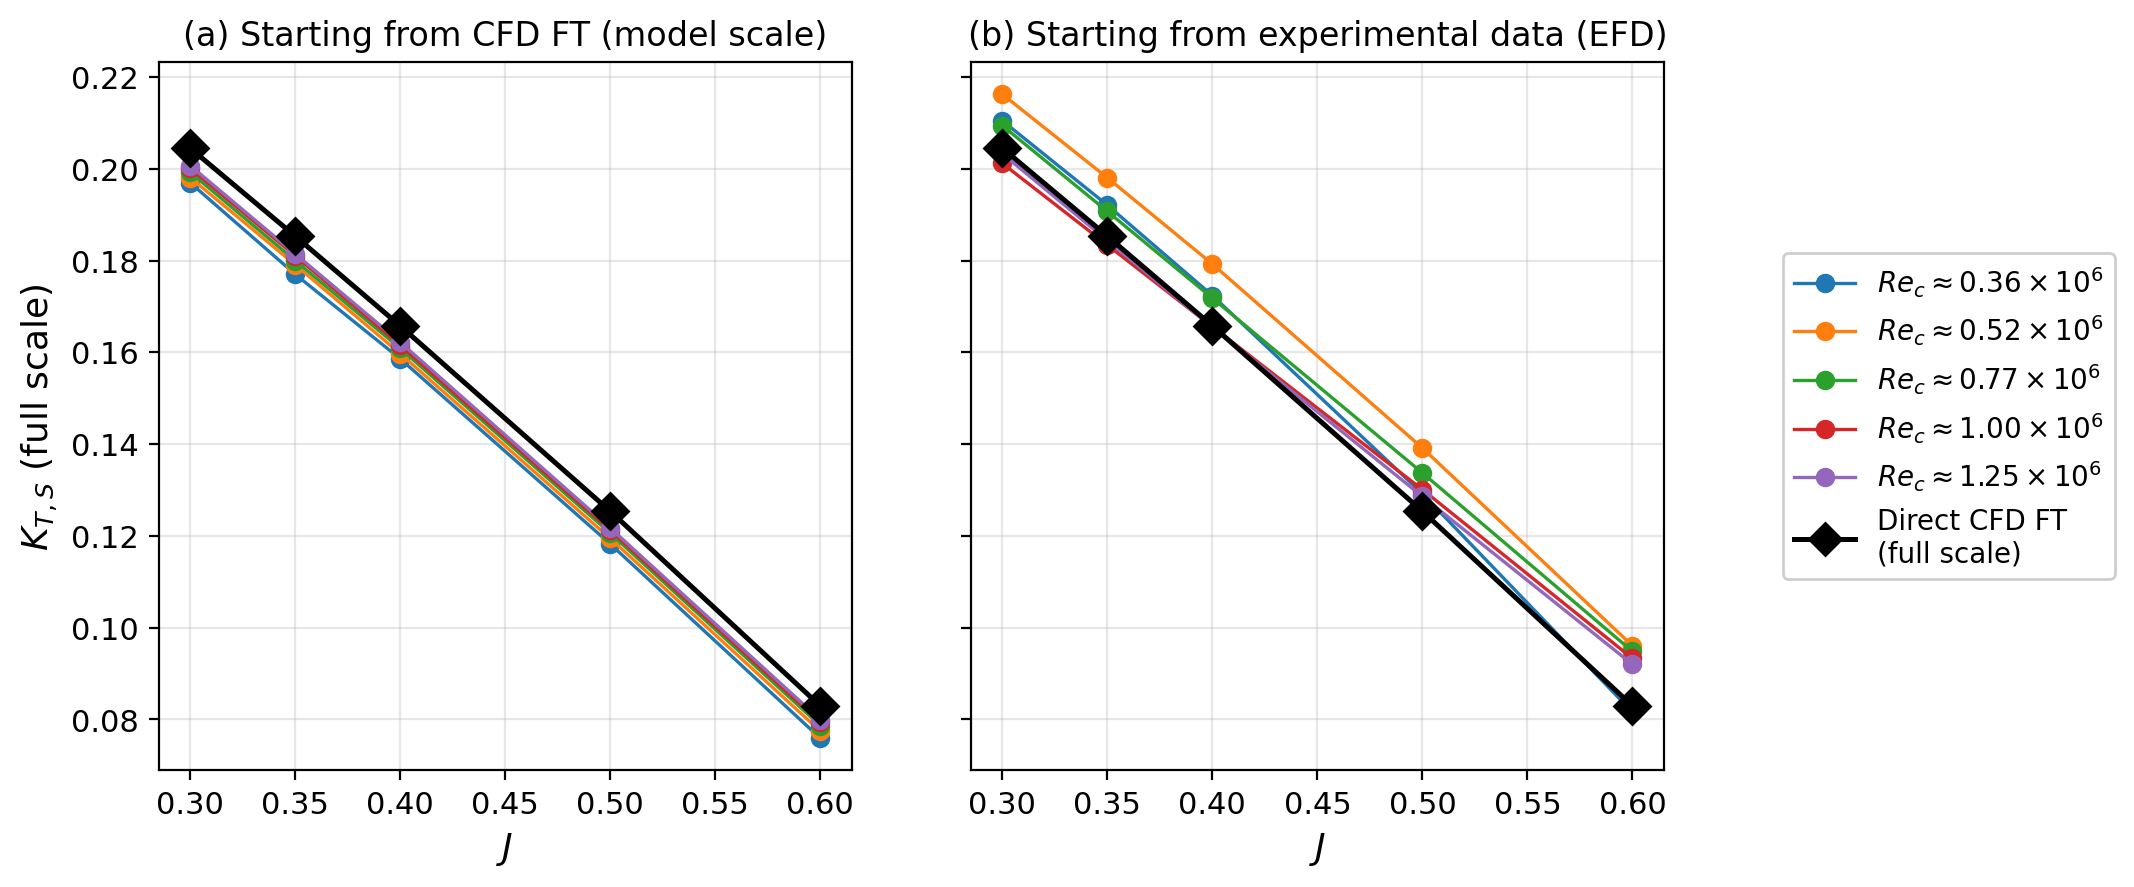
\includegraphics[width=\textwidth]{images/fig_ittc78_vs_cfd_en.png}
    \caption{Predicción de $K_{T,S}$ a escala buque mediante el procedimiento ITTC-78, aplicado a los cinco puntos CFD Fully Turbulent de escala modelo (panel a) y a cada uno de los cinco puntos experimentales de distinto $Re_c$ de modelo (panel b), comparado con el CFD Fully Turbulent resuelto directamente a escala buque (rombos negros).}
    \label{fig:coreana_ittc_vs_cfd}
\end{figure}

Se caracteriza la dispersión de cada columna --el rango de sus cinco predicciones de
escala buque, una por $Re_c$ de ensayo, relativo a la referencia CFD resuelta
directamente a esa escala--:
%
\begin{equation}
\text{dispersión} = 100\,\frac{\max_i K_{T,S}^{i}-\min_i K_{T,S}^{i}}
{K_{T,S}^{\mathrm{CFD}}},
\label{eq:dispersion}
\end{equation}
%
equivalente al rango de los errores de extrapolación de esa columna. El resultado más
relevante de esta comparación no es la media, sino la dispersión de la columna EFD: el
punto de $Re_c = 0.52\times10^6$ --que corresponde casi exactamente
al centro de la ``joroba'' identificada en la Sección~\ref{sec:chichon_antec}, donde el
ensayo registra un $K_T$ anómalamente alto ($0.215$ para $J=0.3$)-- produce por sí
solo un error de extrapolación de $+5.5$ a $+14.5\%$ según el $J$, muy por encima del
resto de los puntos EFD, que en su mayoría predicen razonablemente bien (algunos con
error por debajo del $1\%$). Es decir, la media de la columna EFD ($\sim2.5$--$10.5\%$
según el $J$) esconde un comportamiento muy poco homogéneo: \textbf{el resultado de la
extrapolación depende críticamente de en qué condición de rps se realizó el único
ensayo de túnel disponible}, y si esa condición cae dentro del rango transicional, el
error puede duplicarse o triplicarse respecto de un punto vecino a Reynolds apenas
distinto. Este es precisamente el riesgo práctico señalado en la
Sección~\ref{sec:chichon_antec}: un ensayo de modelo único, realizado sin conocer a
priori si su $Re_c$ cae dentro de la joroba, puede producir una extrapolación ITTC-78
con un error varias veces mayor al que se obtendría con una condición de ensayo apenas
distinta. La brecha se agrava en las condiciones descargadas ($J=0.50$--$0.60$), donde
la propia amplitud de la joroba experimental es mayor (Sección~\ref{sec:coreana_resultados}).

La columna Fully Turbulent, en cambio, es mucho más estable entre puntos para cada $J$
(rango de apenas $2$--$3$ puntos porcentuales dentro de cada columna) pero exhibe un
sesgo sistemático que se profundiza con la descarga del propulsor, de $-2.0\%$ en las
condiciones más cargadas hasta $-10.0\%$ en $J=0.60$, en los cinco puntos y los cinco
$J$ calculados: el ITTC-78, al corregir solo fricción, subestima de forma consistente
el verdadero $K_T$ a $Re_c \approx 1.589\times10^7$. Esta es
la misma conclusión ya obtenida para la B4-60 en la Sección~\ref{sec:helices_ittc78},
ahora confirmada para una segunda geometría y en presencia de un modelo de turbulencia
sin ningún componente transicional.

\subsection{Fracción de presión del efecto de escala del P206}
\label{sec:coreana_fp_correccion}

El sesgo sistemático de la columna Fully Turbulent en la Tabla~\ref{tab:ittc_efd_ft}
es consistente con la conclusión de la Sección~\ref{sec:helices_descomposicion}: el
ITTC-78 ignora la componente de presión del efecto de escala. Para cuantificar esa
componente en el P206 se recurre directamente a la descomposición de fuerzas sobre la
pala, sin inferencias indirectas.

\paragraph{Descomposición directa en dos condiciones de escala buque.} Se dispone de dos
simulaciones completamente turbulentas del mismo propulsor agrandado a $D=6$~m: ambas
corresponden a la misma escala geométrica --con la malla de modelo escalada de manera
uniforme--, y lo que cambia entre ellas es la velocidad de giro, elegida para alcanzar
dos números de Reynolds de escala buque distintos a igual $J$. La primera, a $n=0.80$~rps,
da el $Re_c$ más alto ($Re_c\approx1.589\times10^7$, Tabla~\ref{tab:d6m_resultados}); la
segunda, a $n=0.25$~rps, da un $Re_c$ intermedio entre el de escala modelo y aquel
($Re_c\approx4.97\times10^6$, Tabla~\ref{tab:reint_resultados}), calculado de forma
independiente. Sobre cada uno,
tomando la condición de modelo completamente turbulenta como referencia, la fracción de
presión del efecto de escala se mide directamente como
$f_p=\Delta K_{Tp}/\Delta K_T=\Delta K_{Tp}/(\Delta K_{Tp}+\Delta K_{Tf})$ a partir de la
descomposición de fuerzas de OpenFOAM (Ecuación~\ref{eq:adim_helices}).

\begin{table}[htpb]
\centering
\caption{Resultados de la simulación a $Re_c$ intermedio ($D=6$~m, $n=0.25$~rps,
$Re_c\approx4.97\times10^6$), modelo SST completamente turbulento (OpenFOAM).}
\label{tab:reint_resultados}
\begin{tabular}{cccc}
\hline
$J$ & $K_T$ & $K_Q$ & $\eta_0$ \\
\hline
$0.30$ & $0.202732$ & $0.022043$ & $0.4391$ \\
$0.35$ & $0.183646$ & $0.020550$ & $0.4978$ \\
$0.40$ & $0.164096$ & $0.018977$ & $0.5505$ \\
$0.50$ & $0.123811$ & $0.015548$ & $0.6337$ \\
\hline
\end{tabular}
\end{table}

\begin{table}[htpb]
\centering
\caption{Fracción de presión $f_p = \Delta K_{Tp}/\Delta K_T$ obtenida por
descomposición directa de fuerzas (FT vs.\ FT) para las dos condiciones de escala buque
($Re_c\approx1.589\times10^7$ y $4.97\times10^6$), en función de $J$.}
\label{tab:fp_directo}
\begin{tabular}{ccc}
\hline
$J$ & $f_p$ ($Re_c\approx1.589\times10^7$) & $f_p$ ($Re_c\approx4.97\times10^6$) \\
\hline
$0.30$ & $0.931$ & $0.928$ \\
$0.35$ & $0.929$ & $0.927$ \\
$0.40$ & $0.923$ & $0.920$ \\
$0.50$ & $0.914$ & $0.915$ \\
$0.60$ & $0.898$ & $0.904$ \\
\hline
\end{tabular}
\end{table}

La descomposición directa (Tabla~\ref{tab:fp_directo}) arroja $f_p$ entre $0.90$ y $0.93$, decreciente de forma
monótona con $J$, y prácticamente insensible a la escala: los dos puntos difieren en
menos de $0.01$ en todos los $J$, pese a diferir en un factor $3.2$ en la velocidad de
giro. Es también insensible a cuál de los cinco $Re_c$ de modelo se tome como base de la
comparación (dispersión inferior a $0.01$ en todo $J$), de modo que el valor es una
propiedad del salto de escala y no del par particular de puntos de operación elegido. La
única dependencia robusta es la disminución de $f_p$ con el coeficiente de avance $J$: la
fracción de presión del efecto de escala es mayor en condiciones cargadas. En síntesis,
para el P206 el efecto de escala sobre $K_T$ es de origen de presión en un $90$--$92\%$,
de modo que la fricción --lo único que corrige el ITTC-78-- aporta apenas la fracción
restante.

\paragraph{Comparación con otras geometrías.} Este valor se ubica muy por encima del de
las hélices convencionales de área expandida moderada y muy cerca del de la hélice
geométricamente más parecida al P206. Por un lado, la B4-60 ($A_E/A_0=0.60$, sin skew),
analizada en la Sección~\ref{sec:helices_escala}, presenta $f_p\approx0.69$--$0.77$; un
valor análogo se obtiene para la VP1304 convencional ($A_E/A_0=0.779$) a partir de las
cifras de \citet{gallotti2026}. Por otro lado, el P1727 del mismo trabajo --con $Z=4$,
$A_E/A_0=0.444$ y $c/D_{0.7R}=0.236$, prácticamente idénticos a los del P206
($A_E/A_0=0.431$, $c/D_{0.7R}=0.234$)-- arroja, por descomposición directa de fuerzas,
$f_p\approx0.88$ en el rango de carga de interés, también decreciente con $J$. Queda así
un rango físicamente ordenado por el área expandida: las hélices convencionales de área
moderada (B4-60, VP1304) en $f_p\approx0.70$--$0.77$, y las de área reducida (P206 y
P1727) en la banda alta, $f_p\approx0.88$--$0.92$.

El acuerdo entre el P206 y el P1727 es notable porque el P1727 es una geometría de punta
rakeada (\emph{tip-raked}), mecanismo que el P206 no comparte y que a escala buque agrega
una contribución de presión adicional en la región de punta
\citep{Baltazar2021,gallotti2026}. Cabría esperar, por ello, que su fracción sobrepasara
la del P206; sin embargo, ambas caen prácticamente juntas ($0.88$ frente a
$0.90$--$0.92$). Que la similitud en área expandida y cuerda relativa baste para explicar
fracciones tan próximas, pese a la diferencia de rake, indica que el área expandida
reducida --y no el detalle de la punta-- es el factor que gobierna la elevada fracción de
presión de estas hélices. La coincidencia sirve, además, como respaldo externo de
geometría casi idéntica al valor propio del P206 medido aquí.

\subsection{Implicaciones para el diseño de hélices pequeñas y modelos de disco
actuador}
\label{sec:coreana_implicaciones}

Los dos mecanismos caracterizados en este capítulo --el efecto de escala en régimen turbulento y la transición laminar-turbulenta a escala de modelo-- comparten
el mismo punto ciego del procedimiento ITTC-78, que supone que la totalidad del efecto de
escala es friccional. Ambos, sin embargo, arrastran una contribución de presión que ese
procedimiento no representa: para el primero, un $f_p\approx0.90$--$0.92$ implica que una
corrección puramente friccional, por bien calibrada que esté, no puede por construcción dar
cuenta de más del $8$--$10\%$ del efecto real sobre $K_T$; para el segundo, la
descomposición directa muestra que el desfasaje del modelo transicional respecto del
completamente turbulento es mayoritariamente de presión (del orden del $90\%$), y se
manifiesta también en el par.

Esta limitación tiene una consecuencia directa sobre una clase de aplicaciones cada vez más
frecuente: los modelos de disco actuador empleados para representar el propulsor en
simulaciones de autopropulsión o de interacción casco-hélice. Estos modelos toman como
entrada una curva $K_T$-$K_Q$-$J$ --habitualmente la del ensayo de aguas abiertas a escala
de modelo, o su extrapolación ITTC-78-- y devuelven el empuje y el par distribuidos sobre el
disco. Si el propulsor real opera en régimen transicional, como ocurre en ciertas hélices de
bajo número de Reynolds y en los modelos de ensayo, ninguna curva construida bajo la hipótesis completamente
turbulenta lo representa fielmente, y el disco actuador devolverá empuje y par sesgados sin
ningún indicador interno de la inconsistencia. El sesgo no es despreciable: la
Sección~\ref{sec:coreana_resultados} muestra amplitudes de la joroba de hasta el $16\%$ en
$K_T$, y la Sección~\ref{sec:coreana_ittc_efd_ft} una subestimación sistemática de la extrapolación
ITTC-78 de hasta el $8.5\%$. Para las hélices cuyo número de Reynolds de operación real cae dentro del rango
transicional --como las de vehículos submarinos autónomos y operados remotamente (AUV y
ROV) \citep{pawar2019relevance}--, esto sugiere que la caracterización del régimen
transicional no es un refinamiento académico sino una condición para predecir
correctamente las prestaciones a escala real.

\subsection{Conclusiones parciales}

En el propulsor P206 --de área expandida reducida-- la capa límite a escala
de modelo opera en régimen transicional, y el modelo SST completamente turbulento
--poco sensible a $Re_c$, con un crecimiento monótono leve de apenas $2$ a $6\%$ según
la carga-- no alcanza a reproducir el comportamiento experimental
(Sección~\ref{sec:coreana_resultados}). Los ensayos muestran una joroba transicional:
coeficientes muy superiores a la predicción completamente turbulenta a $Re_c$ bajo,
con una amplitud que crece al descargar el propulsor, del $7.1\%$ a $J=0.30$ al
$16.3\%$ a $J=0.60$; la aproximación entre EFD y SST a medida que $Re_c$ crece es
prácticamente completa a $J\leq0.40$ dentro del rango ensayado, pero a $J=0.50$--$0.60$
persiste una brecha de $5$ a $24\%$ incluso en el mayor $Re_c$ disponible. El modelo
SST-LM captura el mecanismo, pero con fidelidad variable --según el $J$ y el nivel de
$Tu$ subestima o incluso sobrepasa la amplitud medida-- y, sobre todo, ningún valor
único de intensidad turbulenta reproduce la forma de la curva en todo el rango: el
$Tu$ que mejor ajusta cambia de una condición de operación a otra, lo que impide
tratarlo como una propiedad transferible del modelo.

La joroba tiene origen predominantemente de presión. La descomposición directa de las
fuerzas SST-LM muestra que el desfasaje respecto del caso completamente turbulento
proviene en su mayor parte de la presión --del orden del $90\%$--, con la fricción
aportando la fracción menor restante; y el par lo confirma: \emph{aumenta} levemente con
el SST-LM, cuando la fricción, que contribuye positivamente al par, solo podría reducirlo
(Sección~\ref{sec:coreana_resultados}). El diagnóstico seccional
(Sección~\ref{sec:coreana_diagnostico}) localiza el efecto de la transición sobre la
fricción --un frente de transición dependiente de $Tu$ y una tensión de corte
marcadamente más radial, cuya fracción radial pasa de $0.19$ en el caso completamente
turbulento a $0.40$--$0.43$ en el SST-LM-- pero muestra que el cambio de presión no
ocurre en el pico de succión (insensible al modelo, por debajo del $3.1\%$): se trata
de una redistribución de carga a lo largo de la envergadura, consistente con el
mecanismo inferido de los ``paint tests''. La transición se manifiesta así de forma
local y nítida en el campo de fricción, mientras que su efecto dominante sobre el
empuje de presión integrado no está localizado.

La calibración de $Tu$ resulta robusta entre solvers --OpenFOAM y StarCCM+
(Sección~\ref{sec:coreana_solvers})-- y consistente con la validación a $D=6$~m
(Sección~\ref{sec:coreana_d6m}). Trasladado a la extrapolación, el procedimiento
ITTC-78, al suponer un efecto de escala puramente friccional, subestima de forma
sistemática la corrección EFD$\rightarrow$buque hasta en un $8.5\%$
(Sección~\ref{sec:coreana_ittc_efd_ft}). La descomposición directa fija la fracción de
presión del efecto de escala del P206 en $f_p\approx0.90$--$0.92$
(Sección~\ref{sec:coreana_fp_correccion}), de modo que una corrección friccional no
puede dar cuenta de más del $8$--$10\%$ del efecto real; el P1727, hélice de área
reducida geométricamente afín, confirma esa banda con $f_p\approx0.88$, muy por encima
del $0.70$--$0.77$ de las hélices convencionales de área moderada.

En conjunto, ambos mecanismos comprometen la fidelidad de las curvas de aguas abiertas
que alimentan los modelos de disco actuador: construidas bajo la hipótesis
completamente turbulenta o extrapoladas con el ITTC-78, sesgan el empuje y el par de
un propulsor que opera en régimen transicional sin ningún indicador interno de la
inconsistencia (Sección~\ref{sec:coreana_implicaciones}). Para las hélices cuyo Reynolds de
operación real cae en el rango transicional --como las de vehículos submarinos autónomos
y operados remotamente (AUV y ROV)--, caracterizar el régimen transicional deja de ser un
refinamiento académico para volverse una condición de la predicción correcta de
prestaciones a escala real.